\chapter{\VBFHBB\, Analysis}\label{c:K}

	After comparing the base constituents of the \VBFHBB\, event between the offline and HLT level and finding them to be similar in behaviour, the specific objects that make up a \VBFHBB\, event can be studied and compared. In this section, the events were required to pass all cuts discussed in Section \ref{es:as} and the designation of the jets as $b_i$, $j_i$ is highlighted in that section.


\section{Cutflow}

	Prior to investigating the core kinematic variables and the more complex kinematic variables used for the Boosted Decision Tree training (Appendix \ref{a:bdt}), the event cutflow for both the Monte-Carlo and real data should be studied to highlight any differences between the event counts. The event counts are given in Table \ref{t:cutflow}, and the ratio of the events is shown in Figure \ref{f:cutflow}.

	\begin{table}[h]
		\caption{Cutflow for the \textit{two-central} \VBFHBB\, events as described in Section \ref{es:as}. The cutflows are given for the online and offline channels in both data and Monte-Carlo along with the percentage of original events.}
		\label{t:cutflow}
		\medskip
		\centering
		\begin{tabular}{c|c|c|c|c}\toprule
			Cut & MC Offline & MC Online & Data Offline & Data Online \\\midrule
			Clean Events & 6229.48 & 6229.48 & 150611000 & 150611000 \\
			Trigger & 6229.48 & 6229.48 & 6679390 &  6679390 \\
			$\geq2$ \textit{loose} \bjets & 503.552  & 467.146 & 2275760 &  2932620 \\
			$\geq2$ light-jets & 483.499  & 417.845 & 2189700 &  2671280 \\
			\textit{Tight} \bjet\, requirement & 330.962  & 288.806 & 1490320 &   1640290 \\
			Forward jet requirement & 51.843   & 40.8484 & 1186610 &  958414  \\
			\ptbb$>160$GeV & 32.7426  & 26.7038 & 309454  &  259411  \\
			\bottomrule
		\end{tabular}
	\end{table}

	\begin{figure}[h]
		\centering
		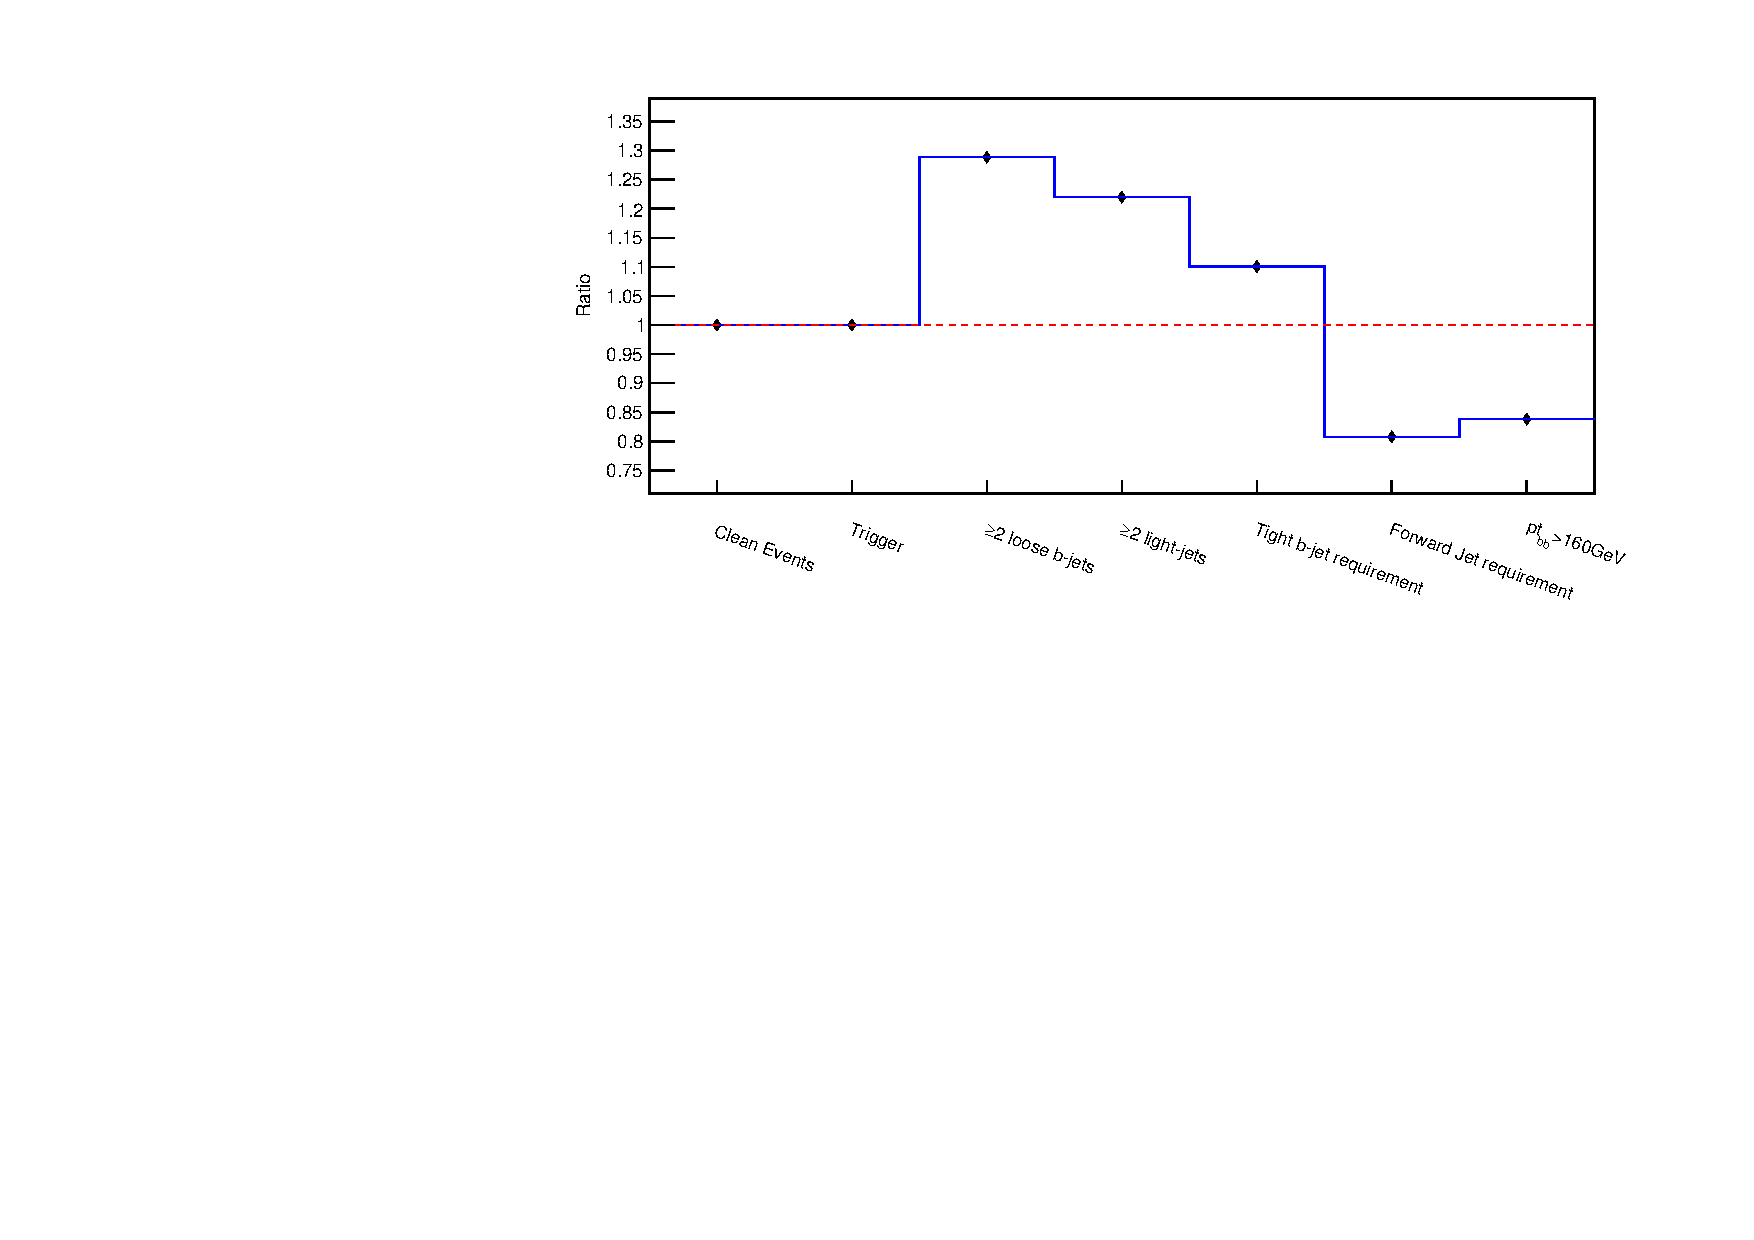
\includegraphics[width=0.75\linewidth]{D_cutflow}
		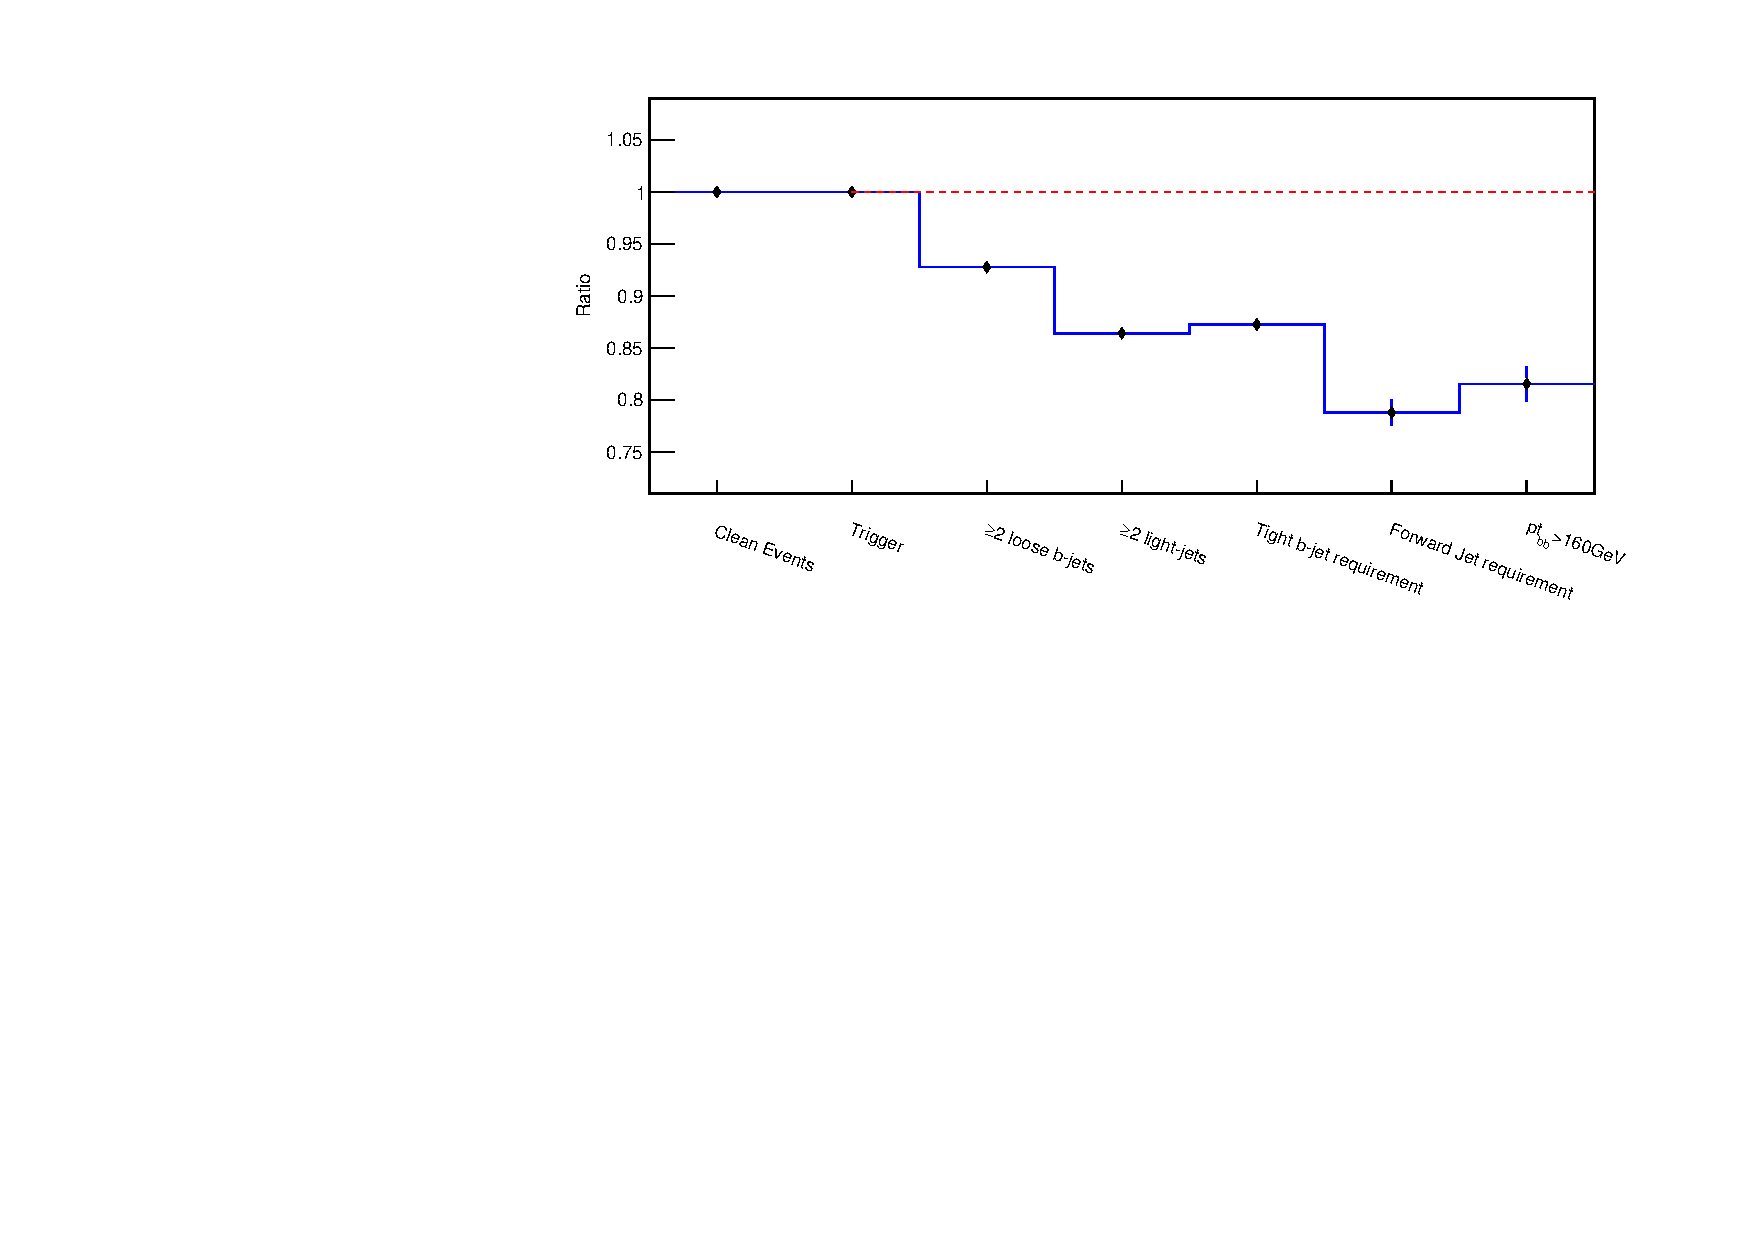
\includegraphics[width=0.75\linewidth]{MC_cutflow}
		\caption{Ratio of the online event count over the offline event count for the real data (top) and Monte-Carlo (bottom) cutflows.}
		\label{f:cutflow}
	\end{figure}




\section{Specific Jet Feature Distributions}

	As the previous chapter showed both \bjets\, and non \bjets\, to be similar for online and offline objects, the kinematic properties of the jets that compose the \VBFHBB\, event are shown to behave similarly.

		\subsubsection{\pt}

			\begin{figure}[h]
				\centering

				\begin{minipage}[h]{0.33\linewidth}
					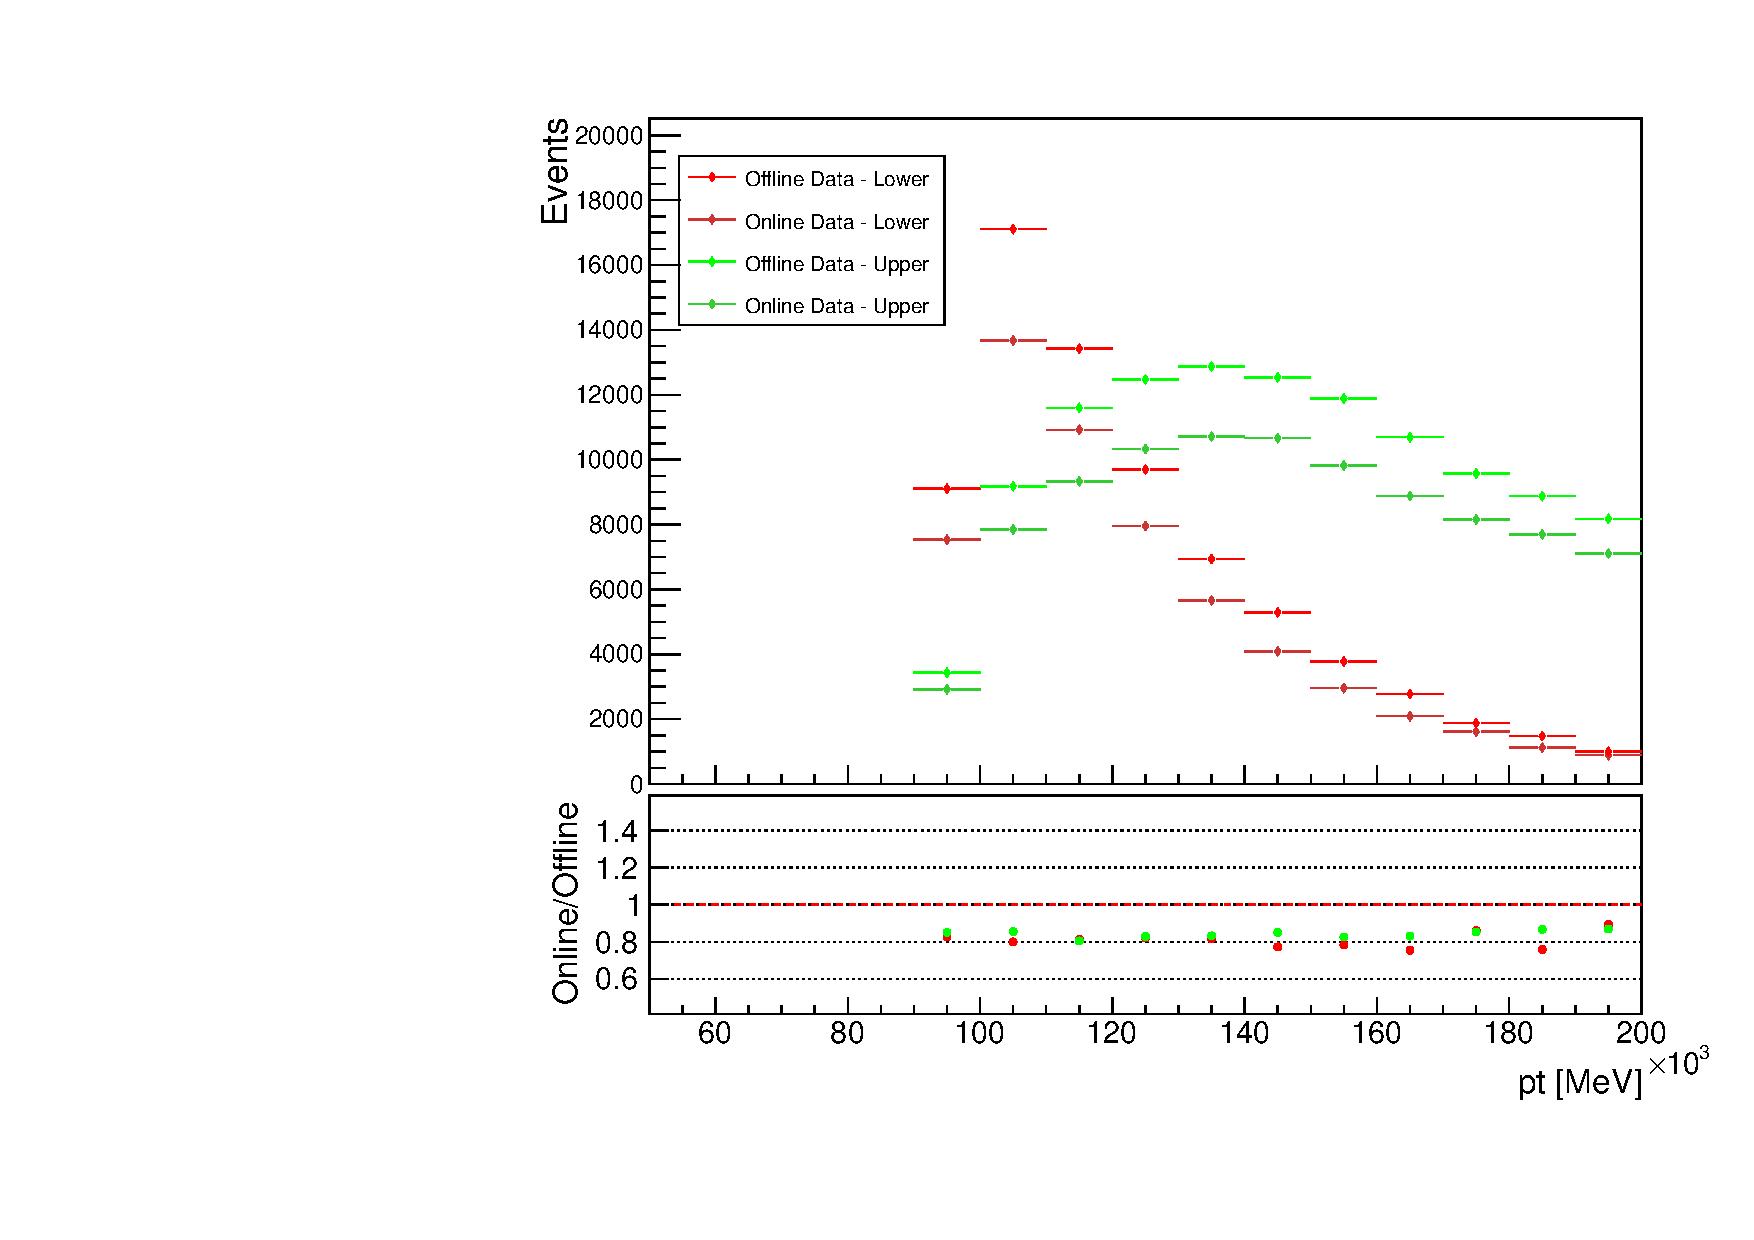
\includegraphics[width=1\linewidth]{pt_bJet1_data_}
				\end{minipage}
				\quad
				\begin{minipage}[h]{0.33\linewidth}
					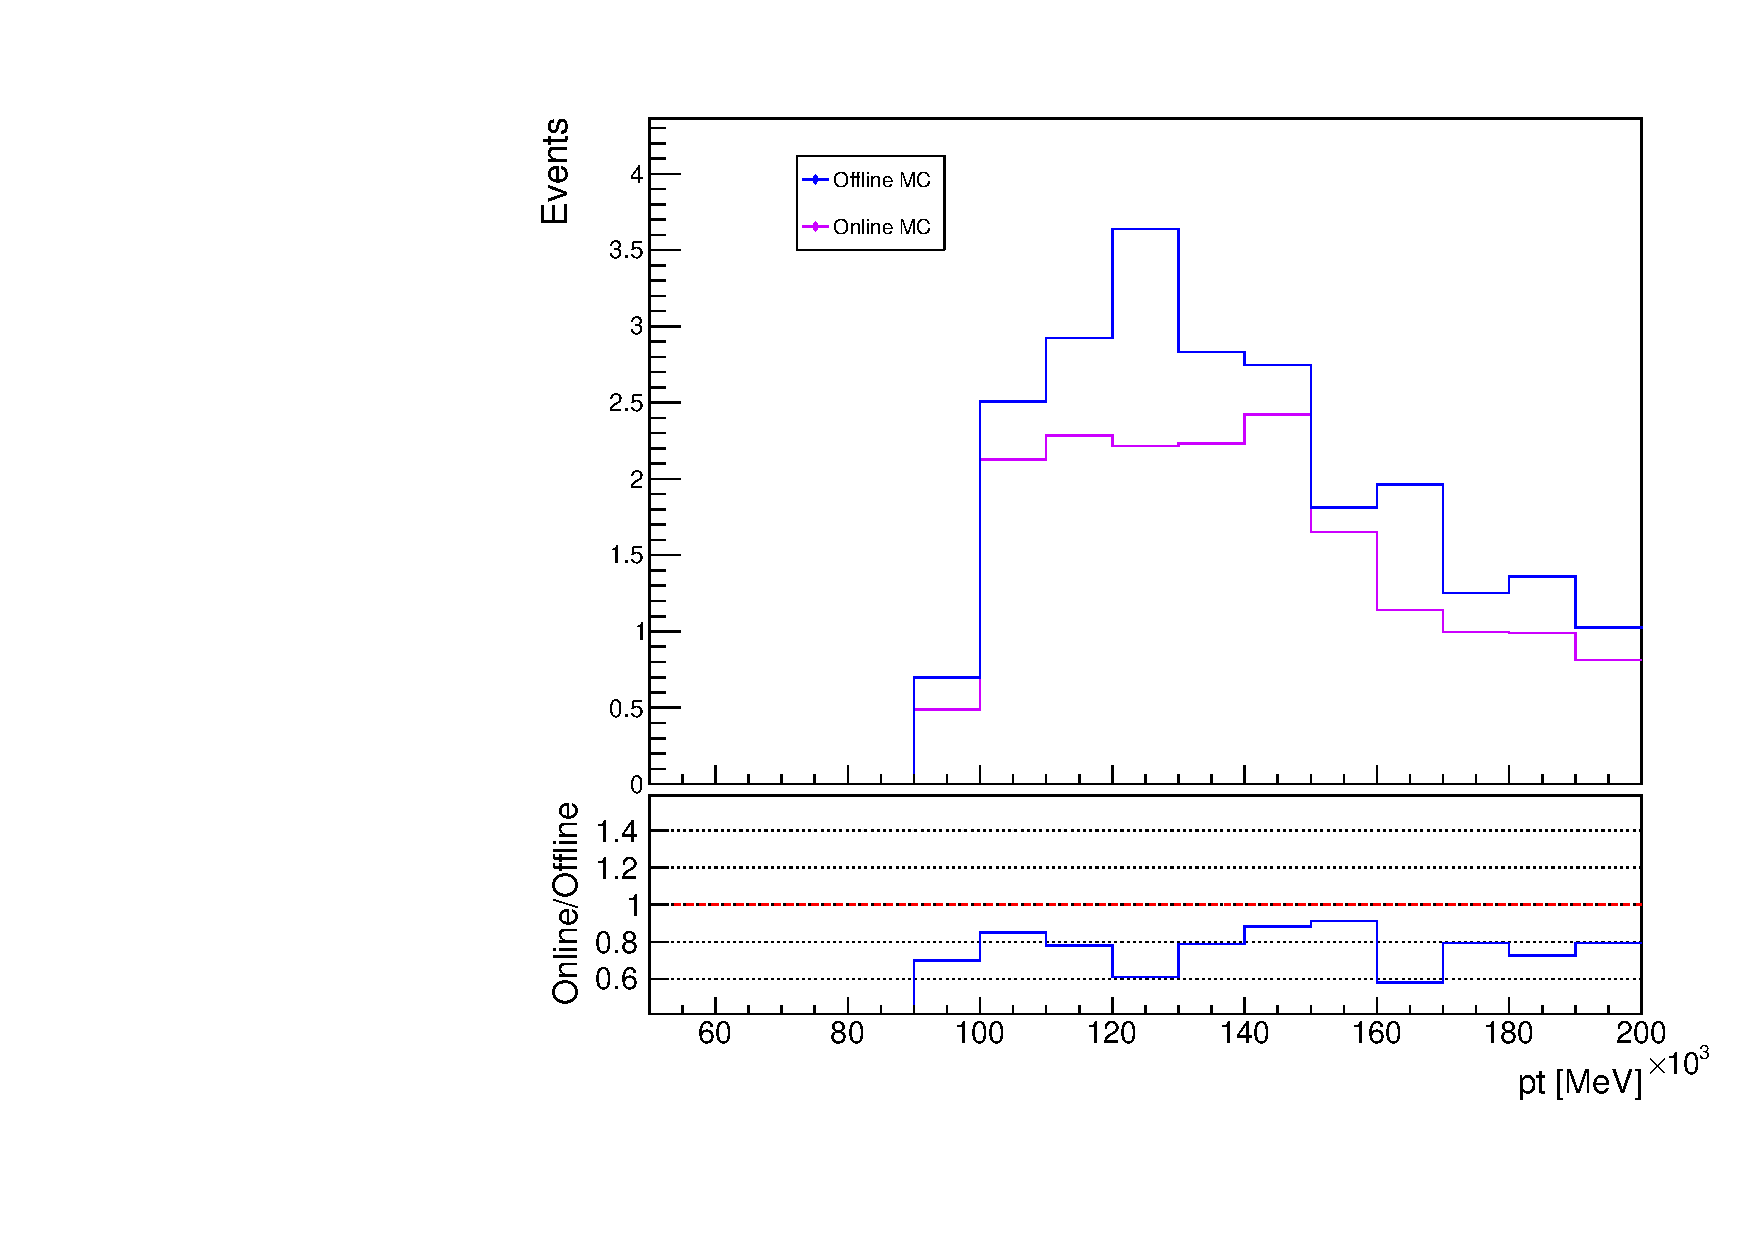
\includegraphics[width=1\linewidth]{pt_bJet1_mc_}
				\end{minipage}

				\begin{minipage}[h]{0.33\linewidth}
					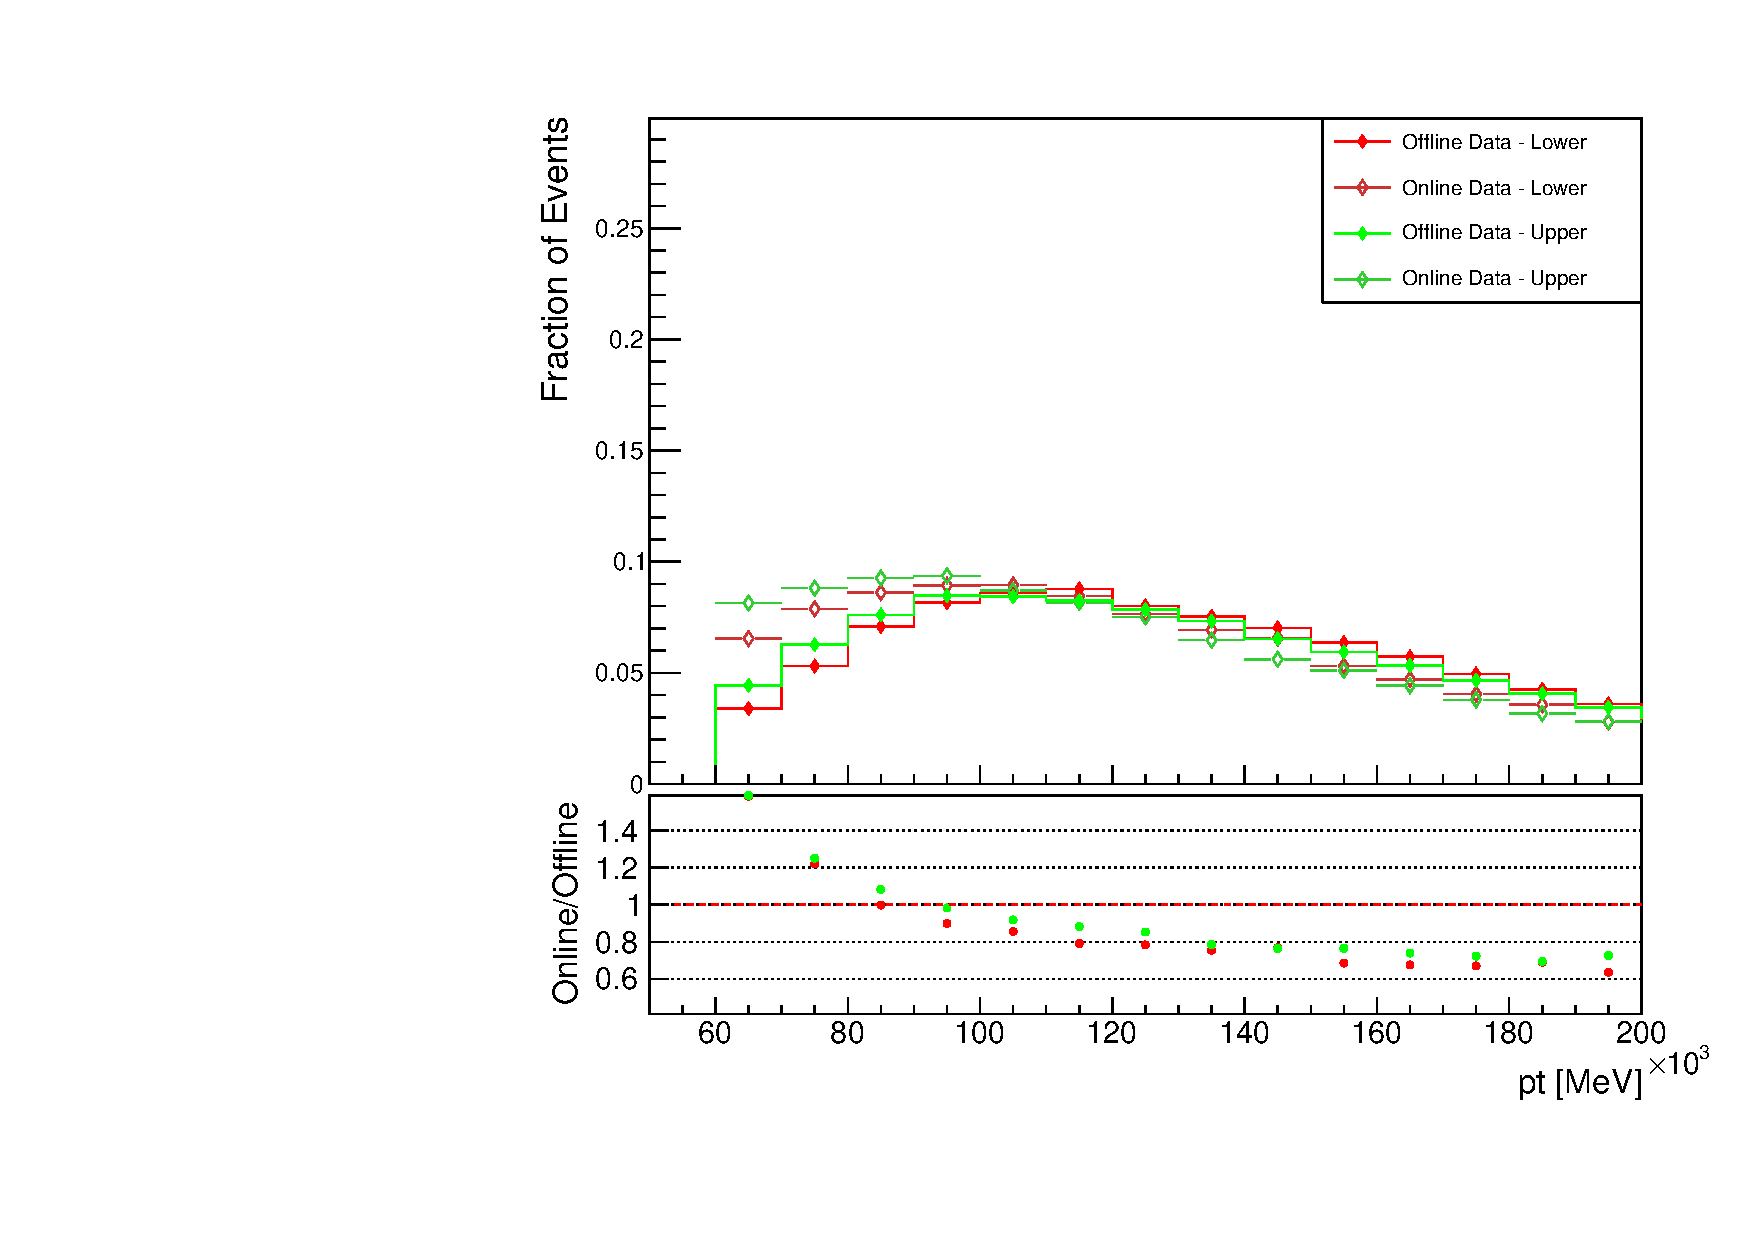
\includegraphics[width=1\linewidth]{pt_lJet1_data_}
				\end{minipage}
				\quad
				\begin{minipage}[h]{0.33\linewidth}
					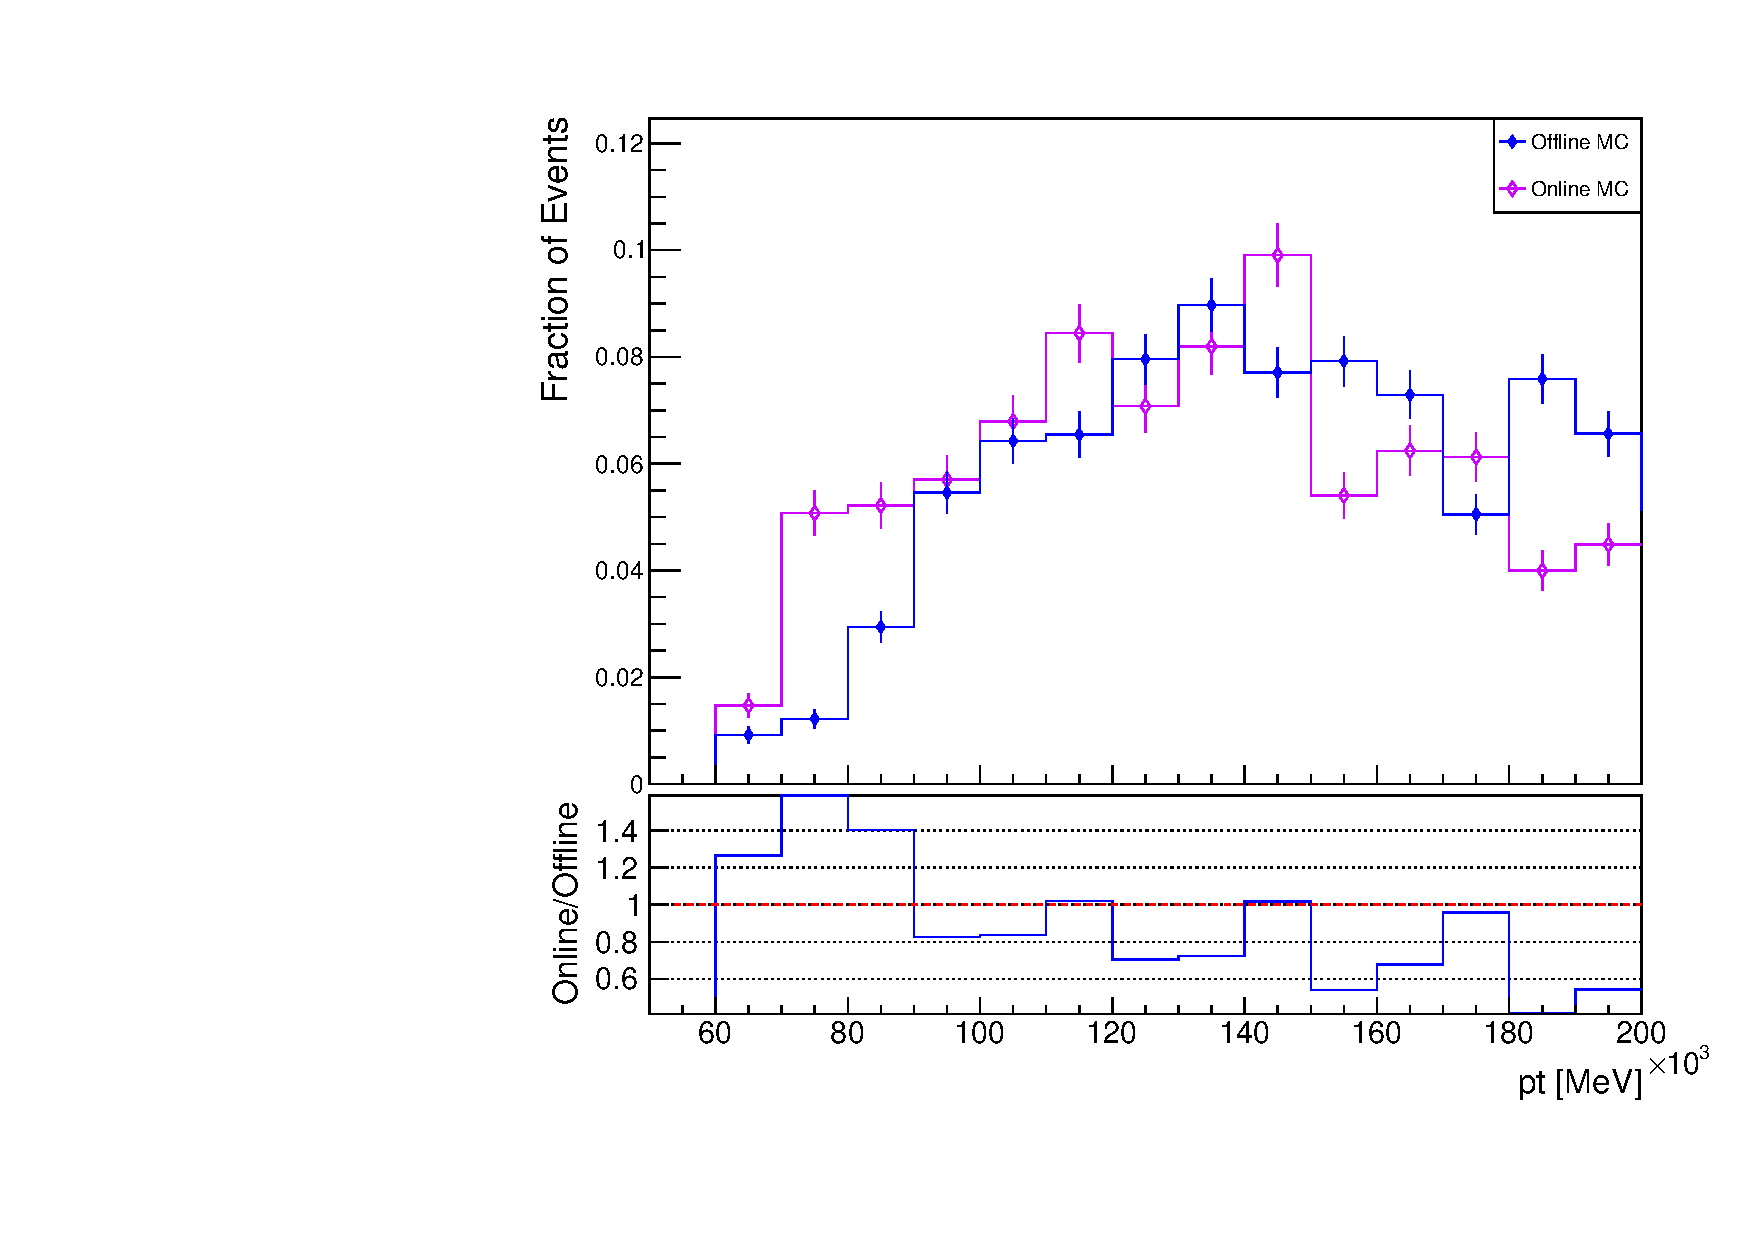
\includegraphics[width=1\linewidth]{pt_lJet1_mc_}
				\end{minipage}

			\end{figure}



			\subsubsection{$\eta$}

				\begin{figure}[h]
					\centering

					\begin{minipage}[h]{0.33\linewidth}
						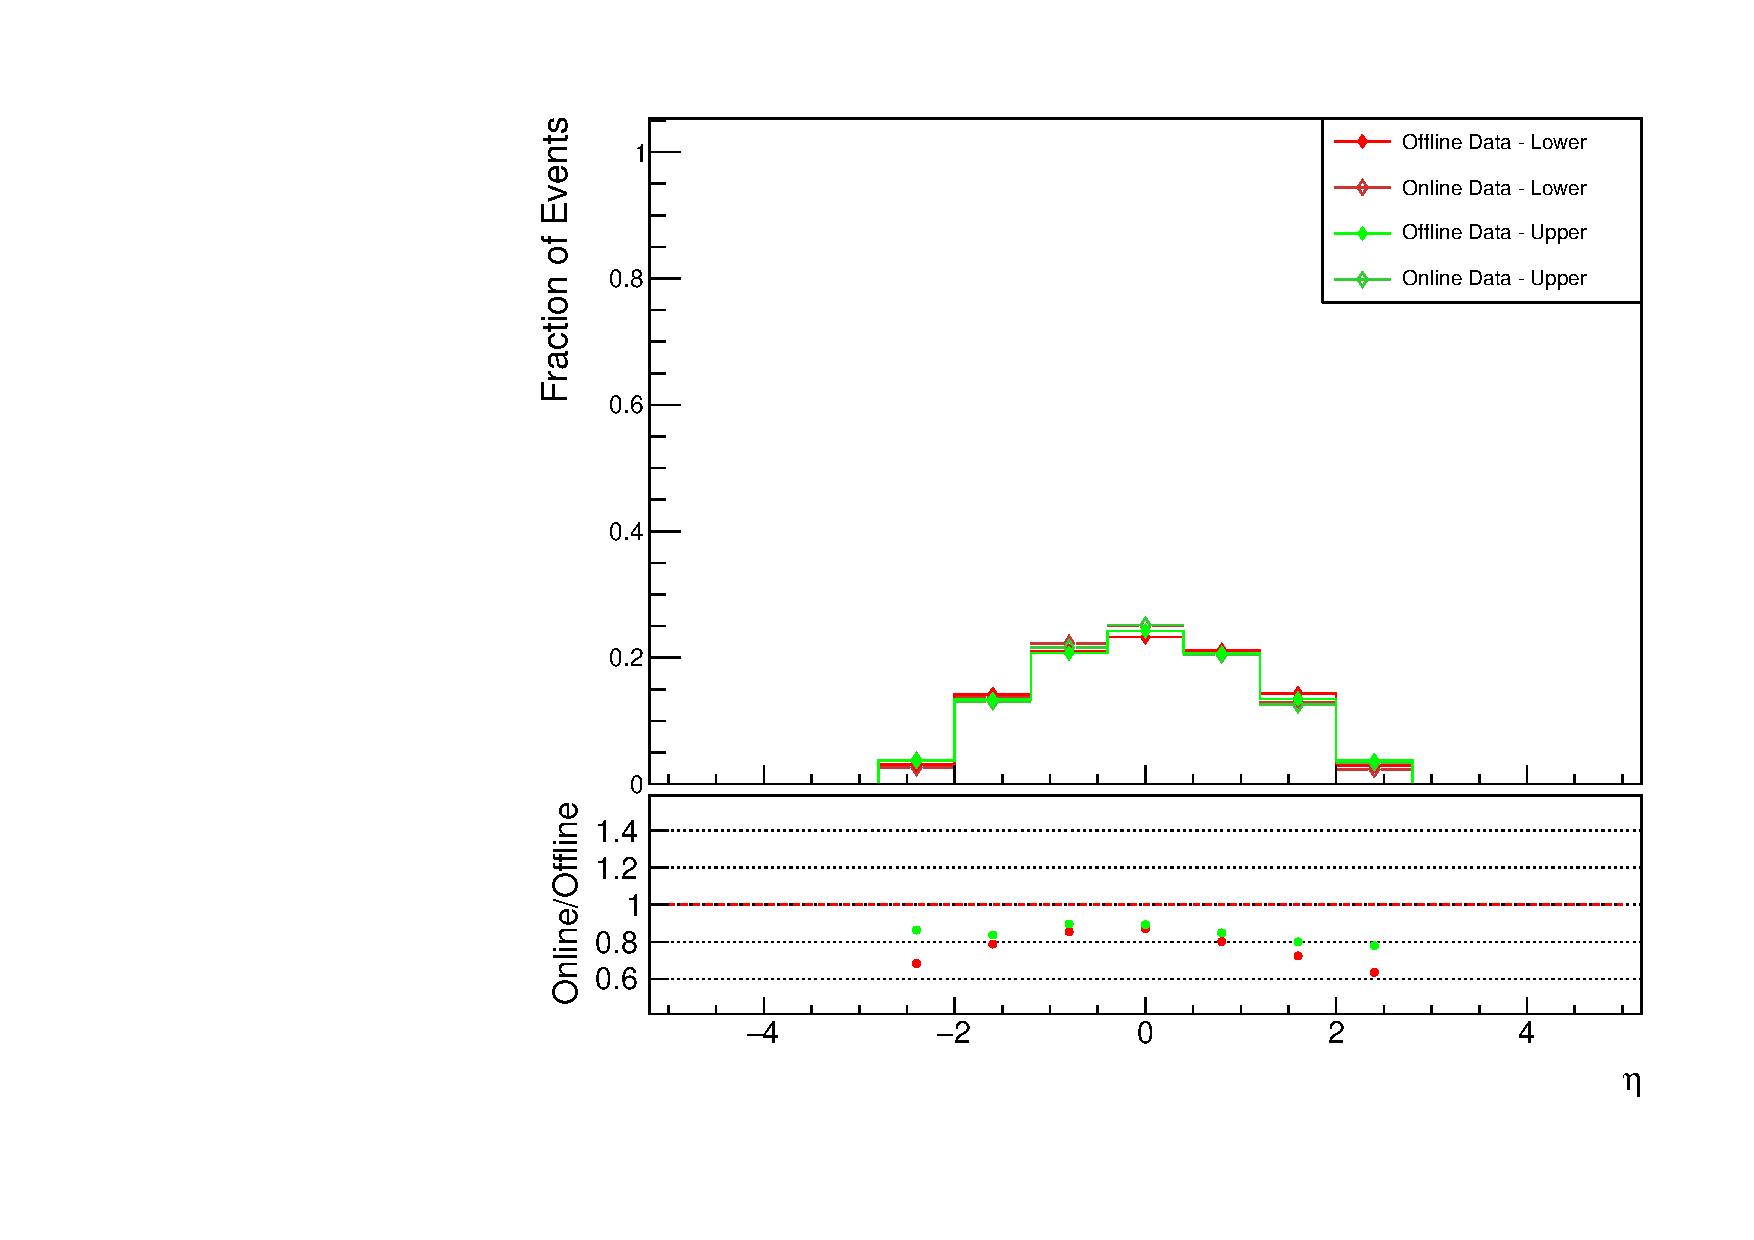
\includegraphics[width=1\linewidth]{eta_bJet1_data_}
					\end{minipage}
					\quad
					\begin{minipage}[h]{0.33\linewidth}
						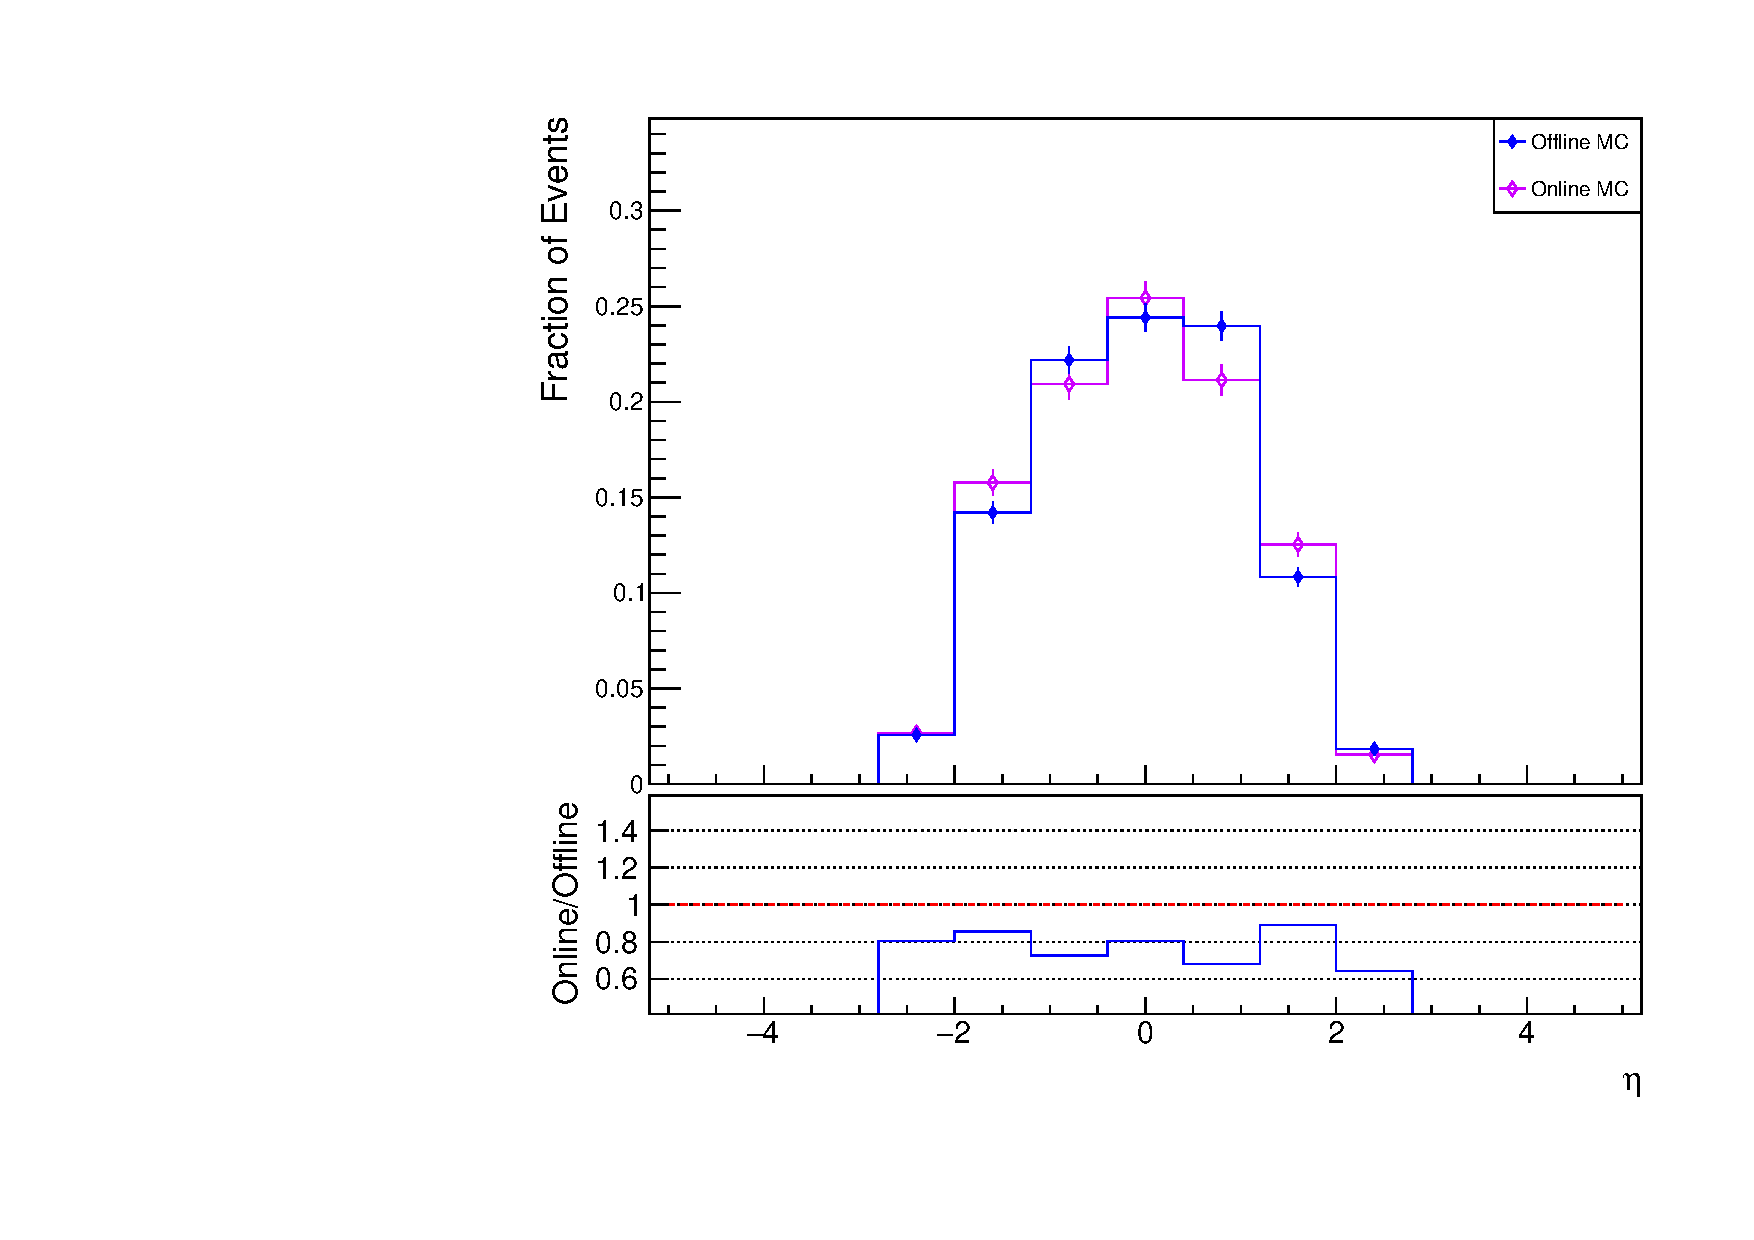
\includegraphics[width=1\linewidth]{eta_bJet1_mc_}
					\end{minipage}

					\begin{minipage}[h]{0.33\linewidth}
						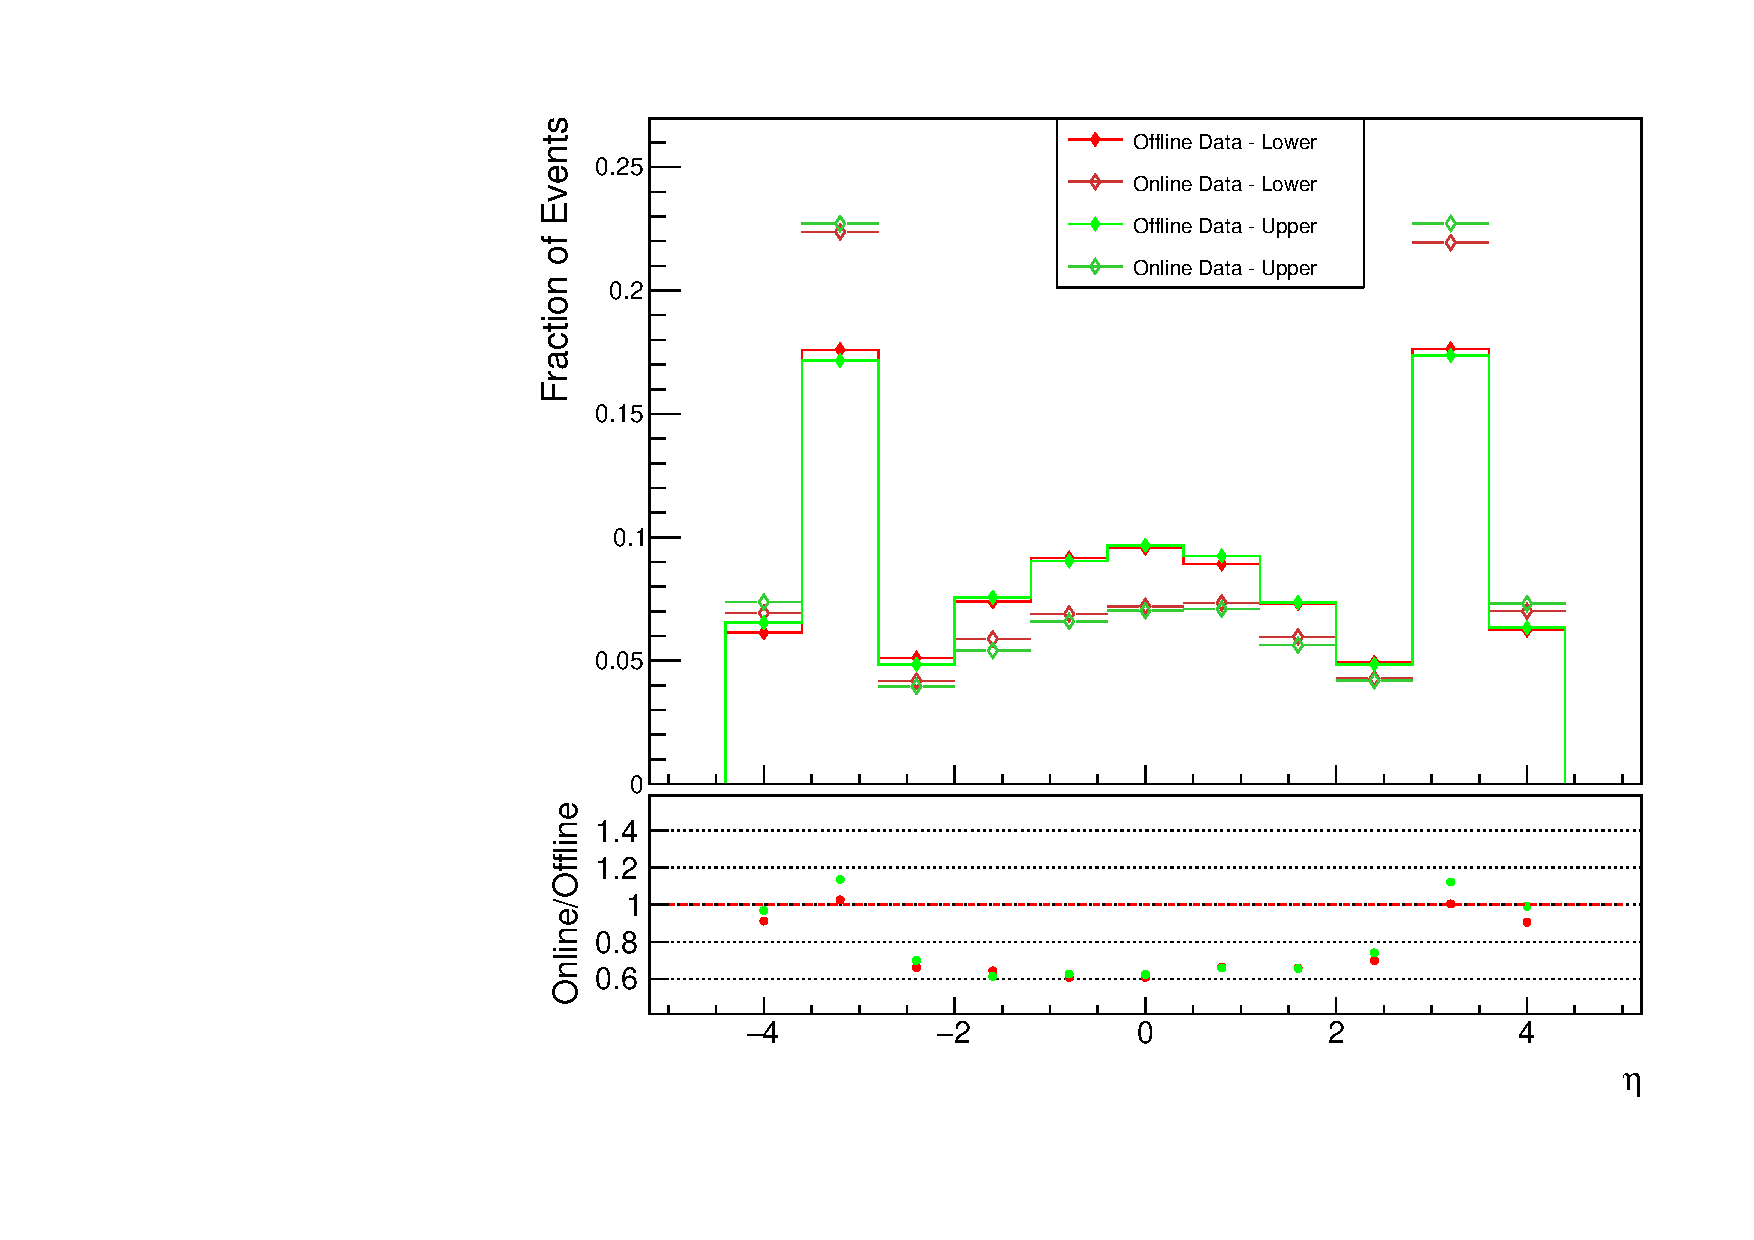
\includegraphics[width=1\linewidth]{eta_lJet1_data_}
					\end{minipage}
					\quad
					\begin{minipage}[h]{0.33\linewidth}
						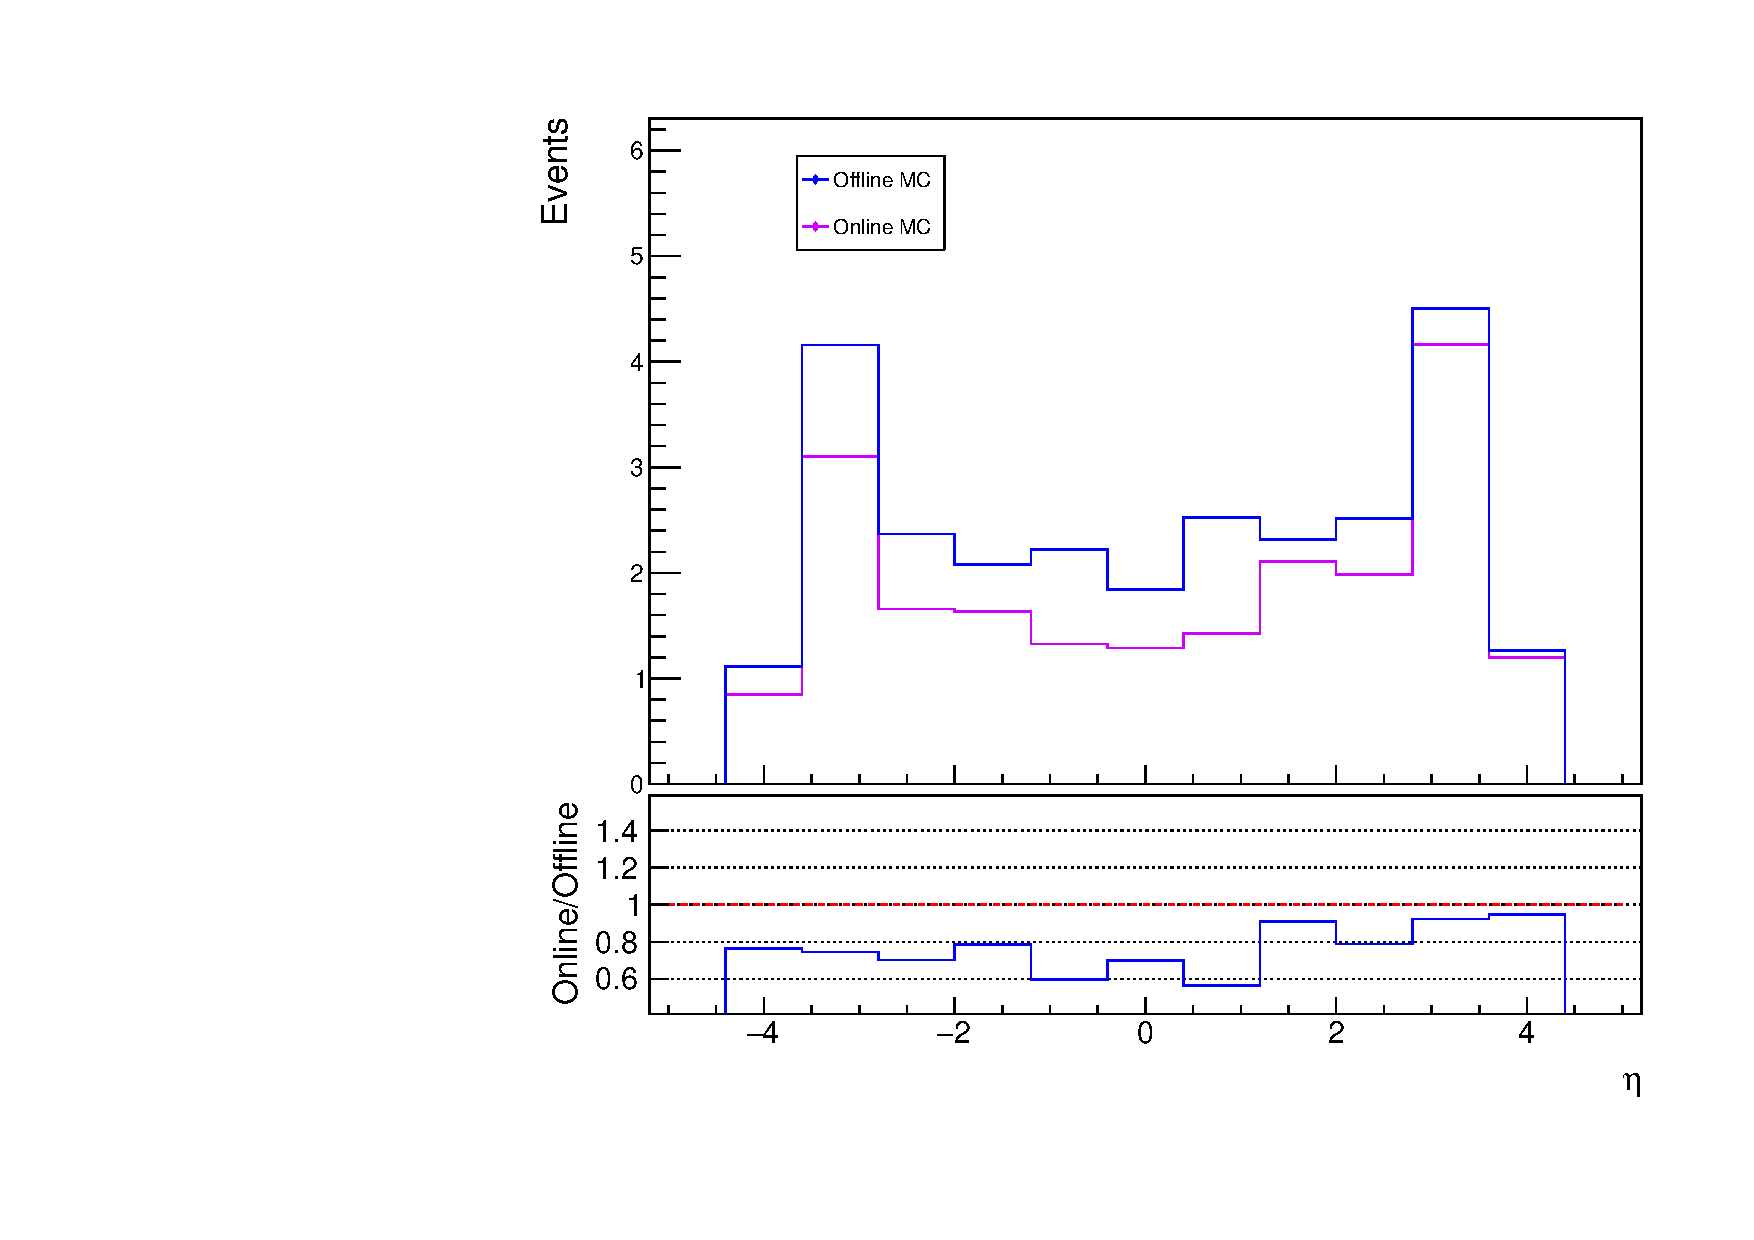
\includegraphics[width=1\linewidth]{eta_lJet1_mc_}
					\end{minipage}
					\label{fig:kin:eta2c4j}
				\end{figure}


\section{BDT Input Variables}

	\begin{itemize}
		\item $M_{jj}$
		\item \pt$_{jj}$
		\item $\cos \theta$
		\item $\Delta\eta_{jj}$
		\item $Max(\eta)$
		\item $\eta*$
		\item $min\Delta R(j_1)$
		\item $min\Delta R(j_1)$
		\item \pt balance
		\item $N_{TRK}(j_1) PV500$ ?
		\item $N_{TRK}(j_) PV500$ ?
	\end{itemize}

		\begin{figure}[h]
			\centering1
			\begin{minipage}[h]{0.45\linewidth}
				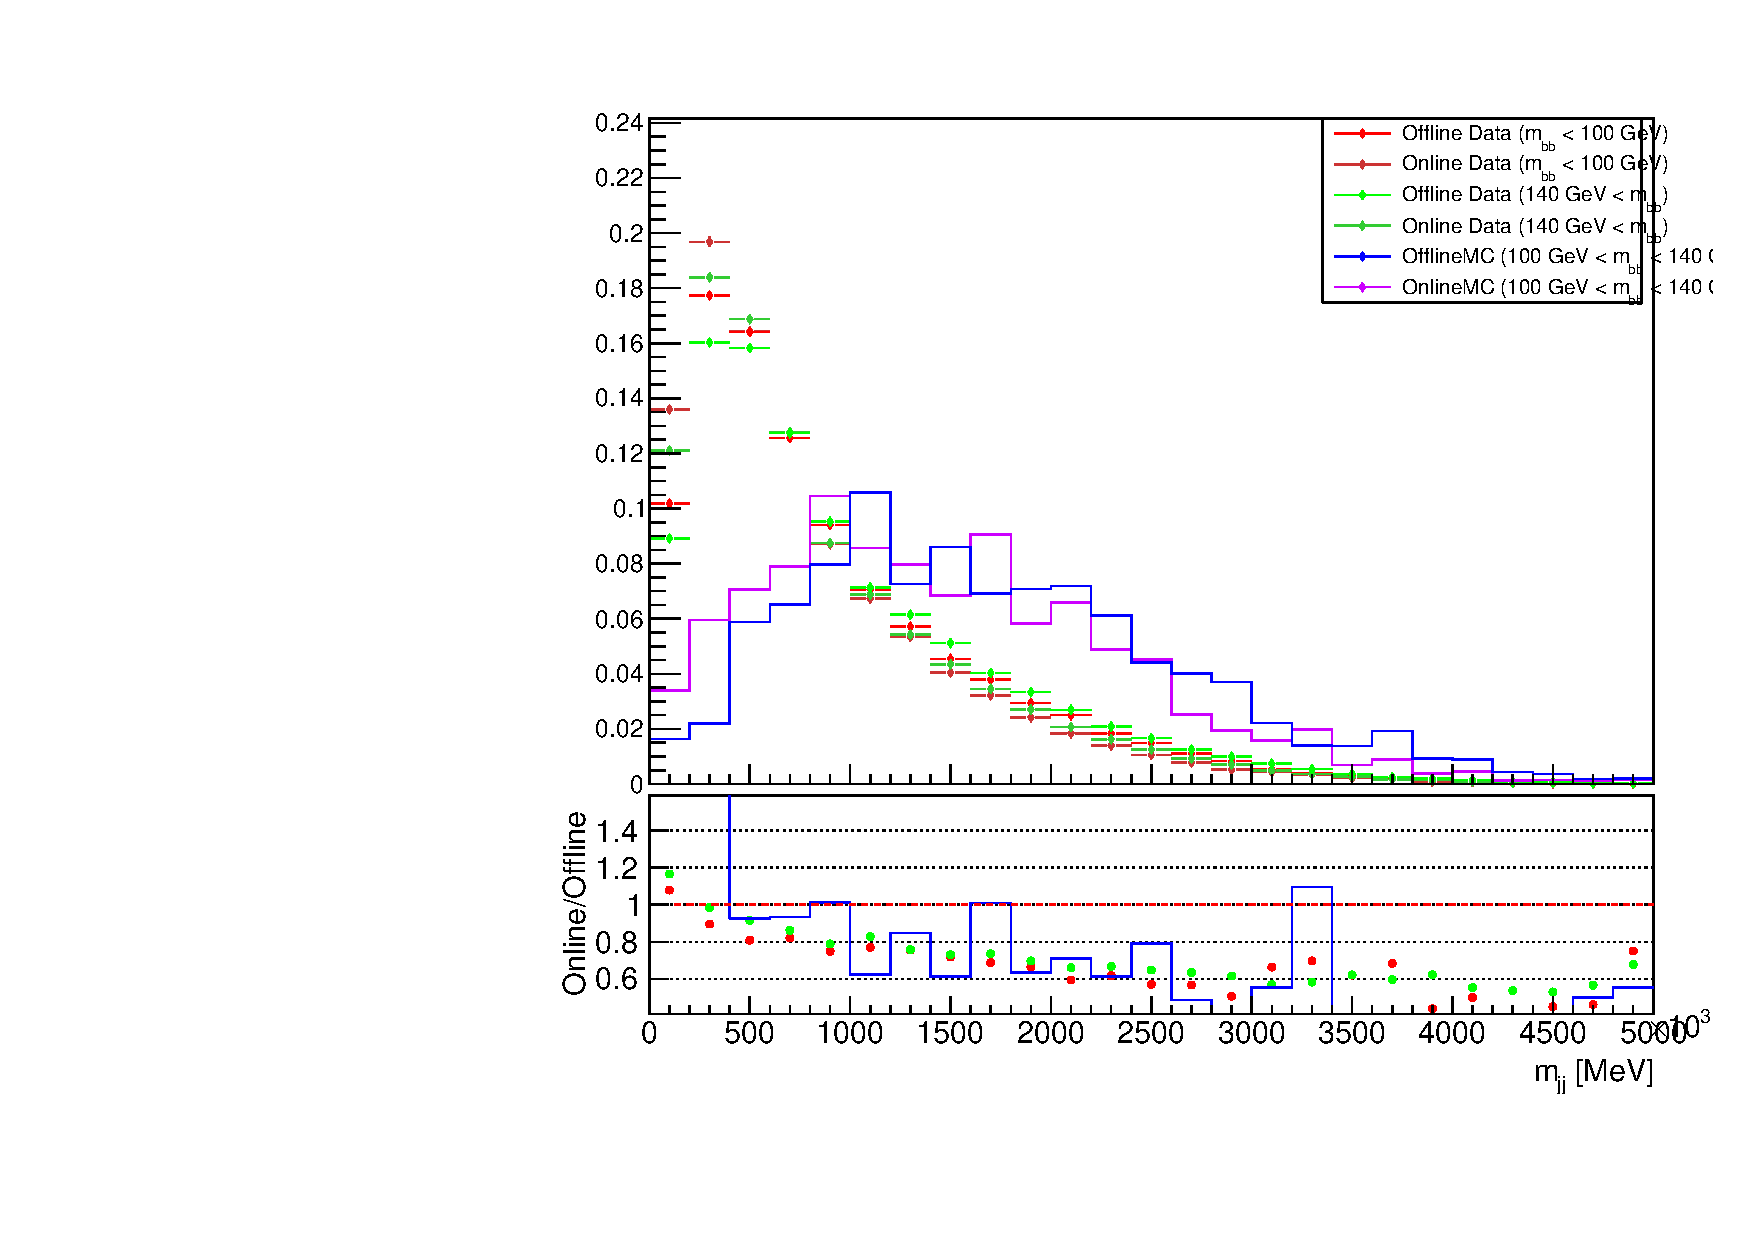
\includegraphics[width=1\linewidth]{mjj}
				\caption{}
				\label{fig:bdtmjj}
			\end{minipage}
			\quad
			\begin{minipage}[h]{0.45\linewidth}
				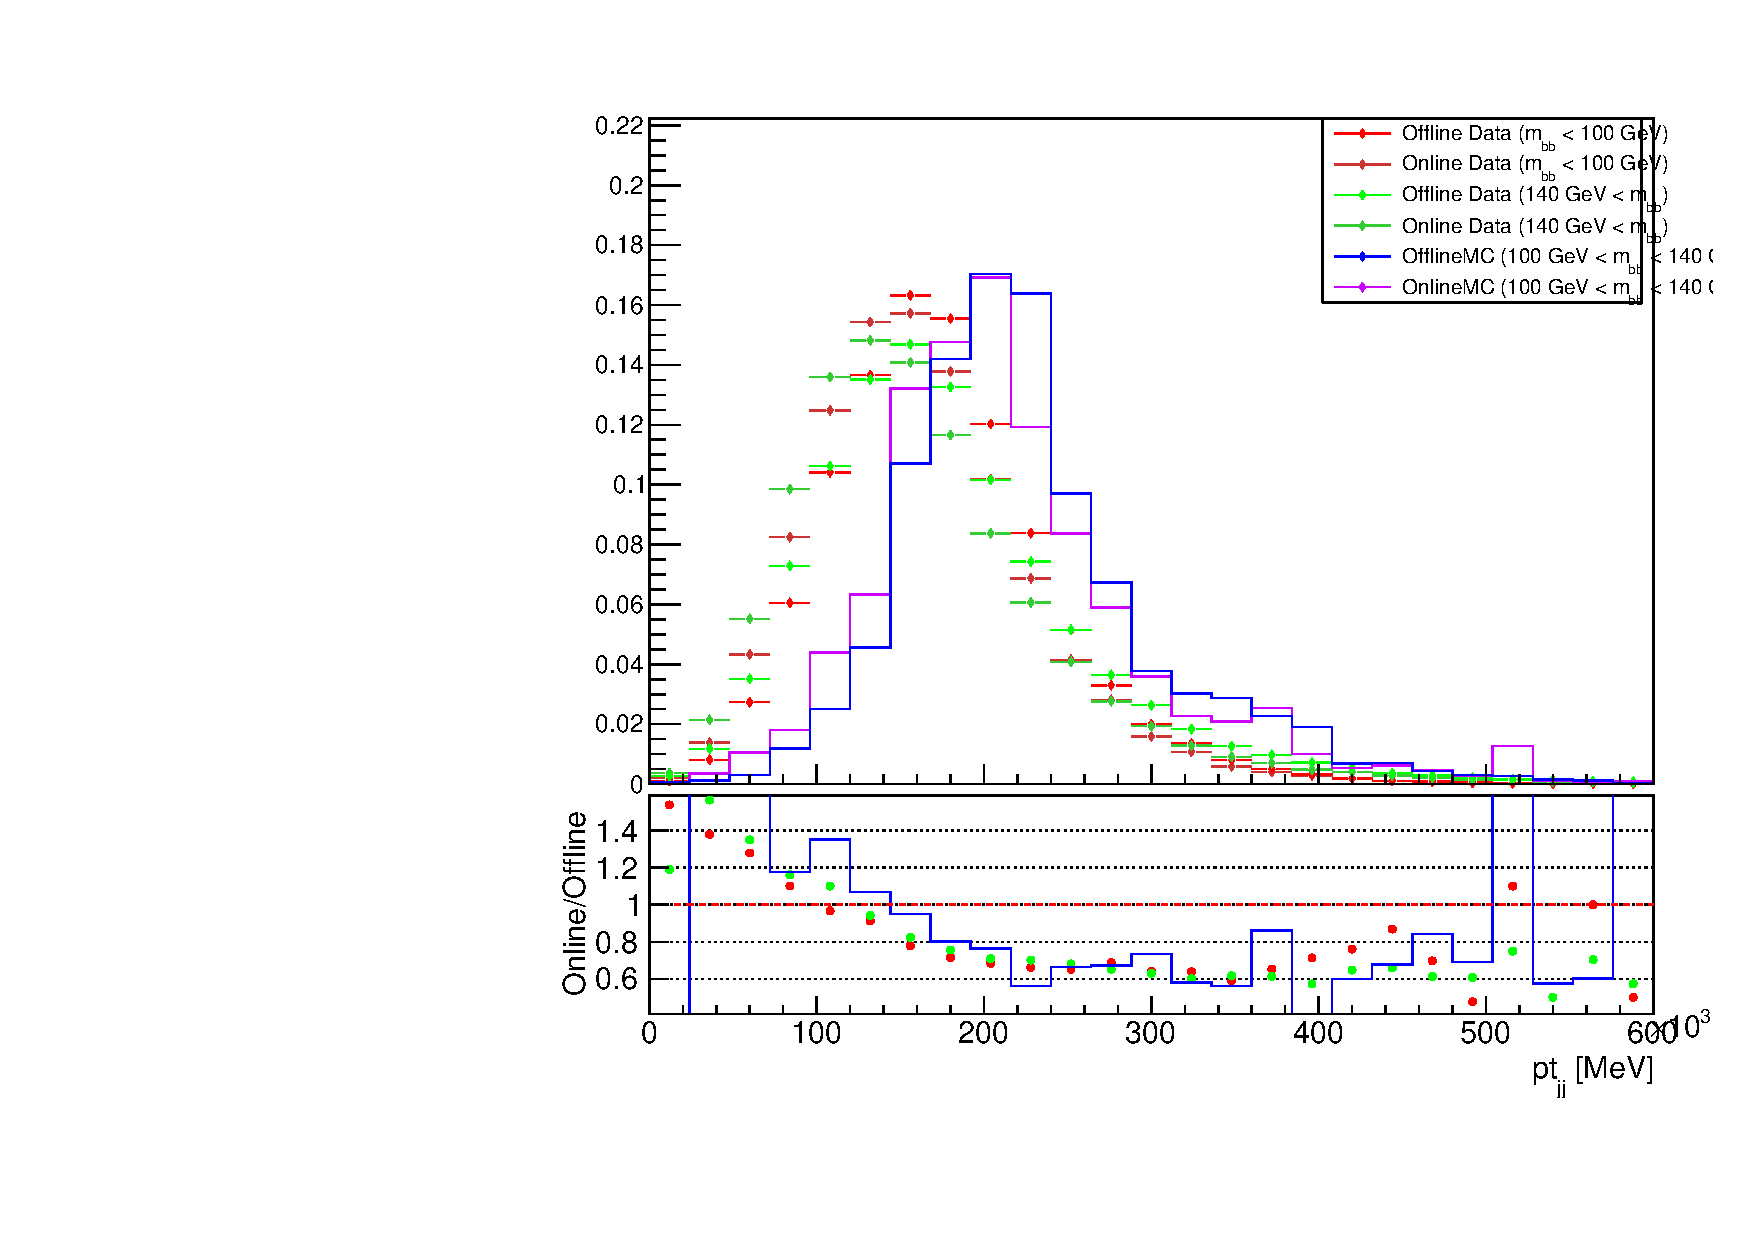
\includegraphics[width=1\linewidth]{ptjj}
				\caption{}
				\label{fig:bdtptjj}
			\end{minipage}
		\end{figure}

		\begin{figure}[h]
			\centering
			\begin{minipage}[h]{0.45\linewidth}
				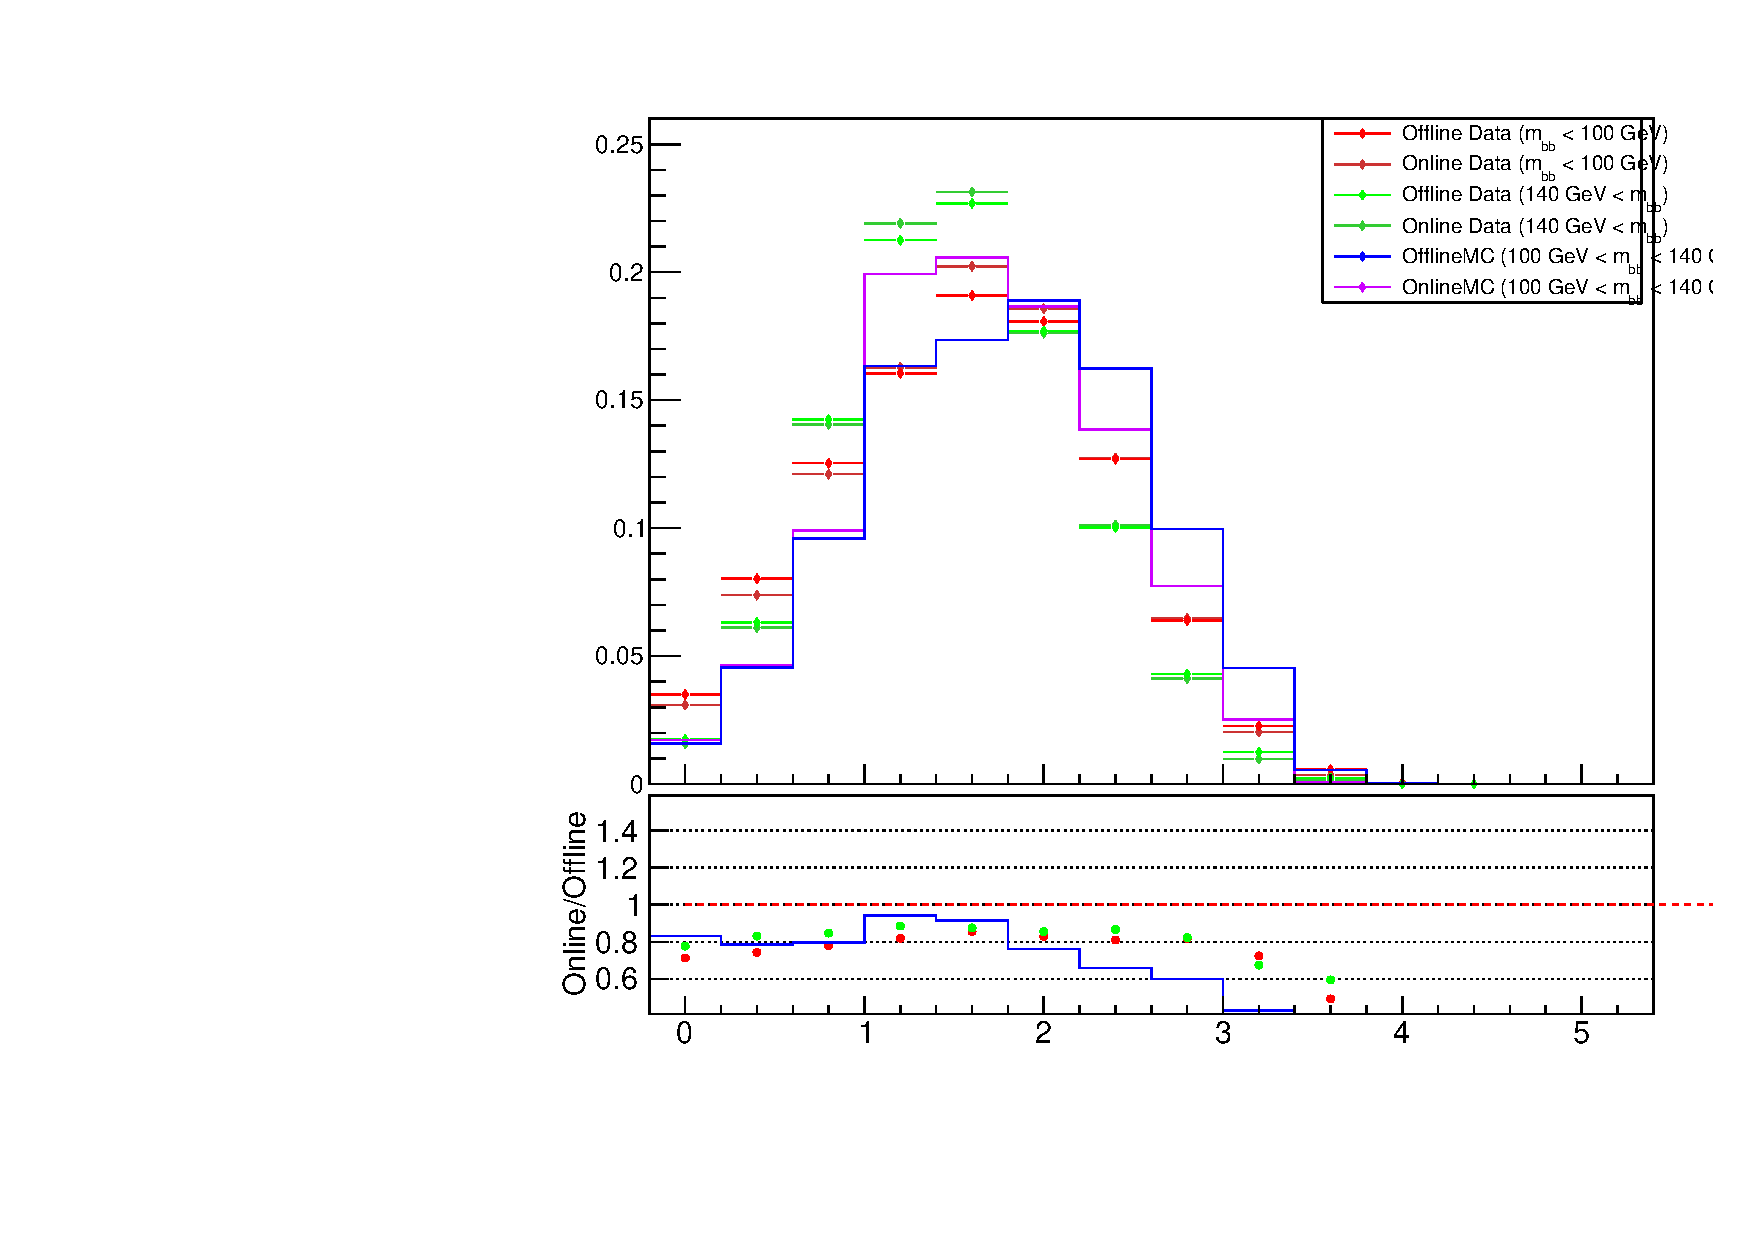
\includegraphics[width=1\linewidth]{etastar}
				\caption{}
				\label{fig:bdtetastar}
			\end{minipage}
			\quad
			\begin{minipage}[h]{0.45\linewidth}
				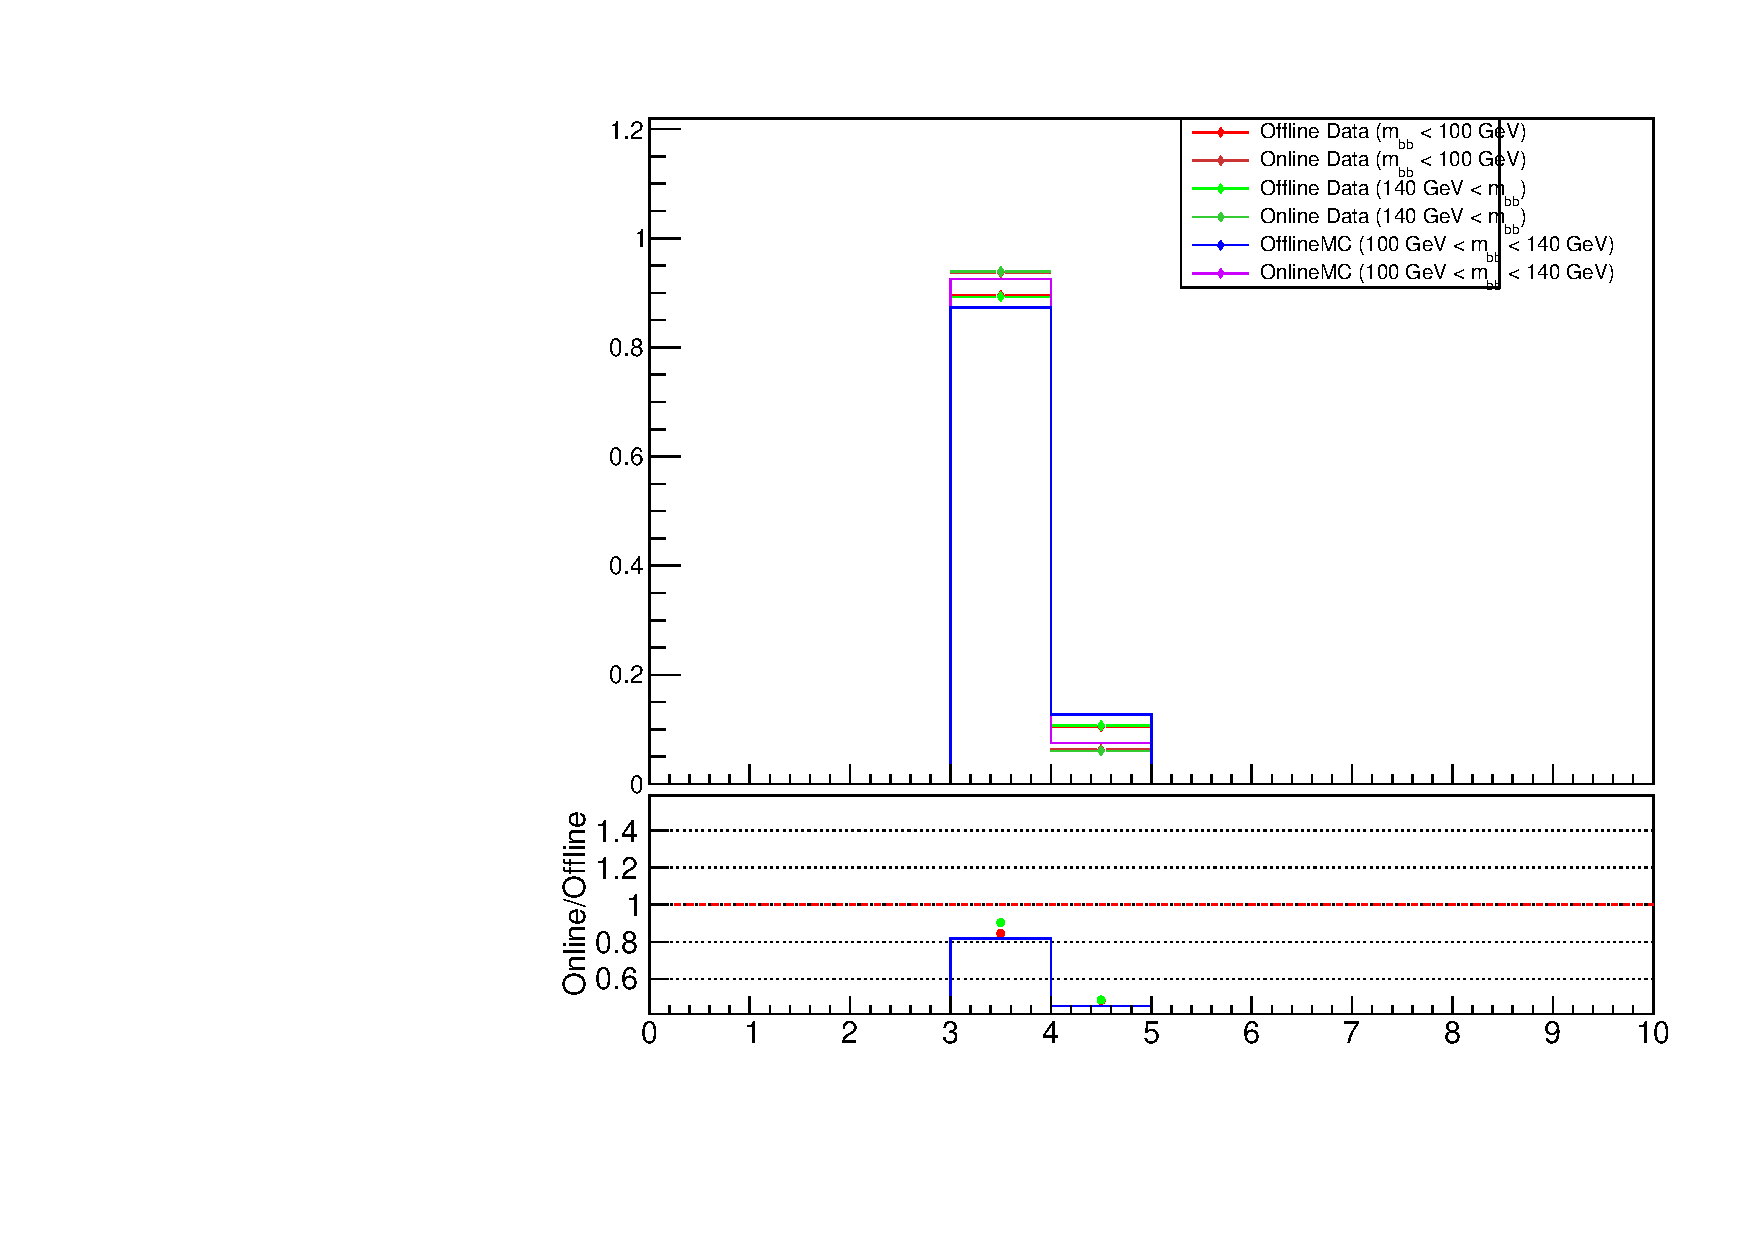
\includegraphics[width=1\linewidth]{maxeta}
				\caption{}
				\label{fig:bdtmaxeta}
			\end{minipage}
		\end{figure}

		\begin{figure}[h]
			\centering
			\begin{minipage}[h]{0.45\linewidth}
				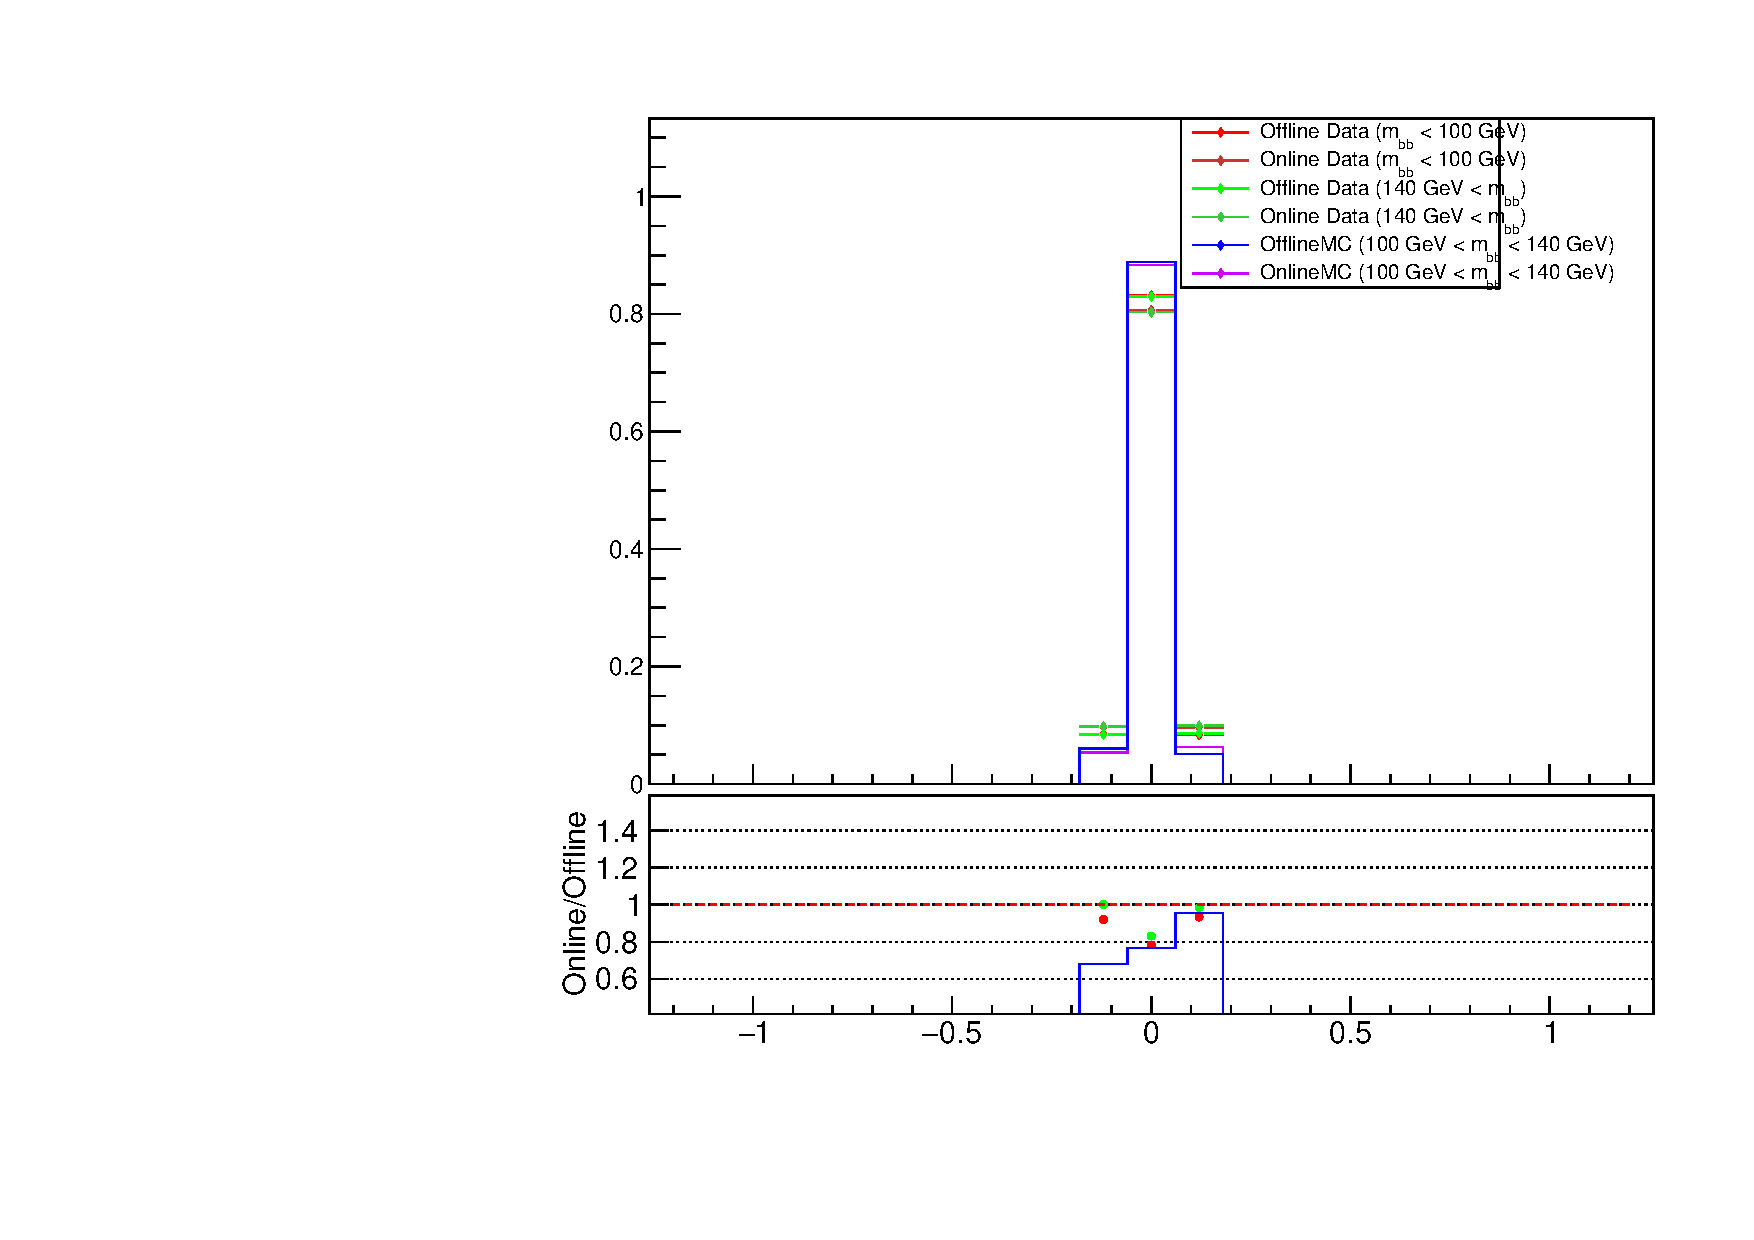
\includegraphics[width=1\linewidth]{costheta}
				\caption{}
				\label{fig:bdtcpostheta}
			\end{minipage}
			\quad
			\begin{minipage}[h]{0.45\linewidth}
				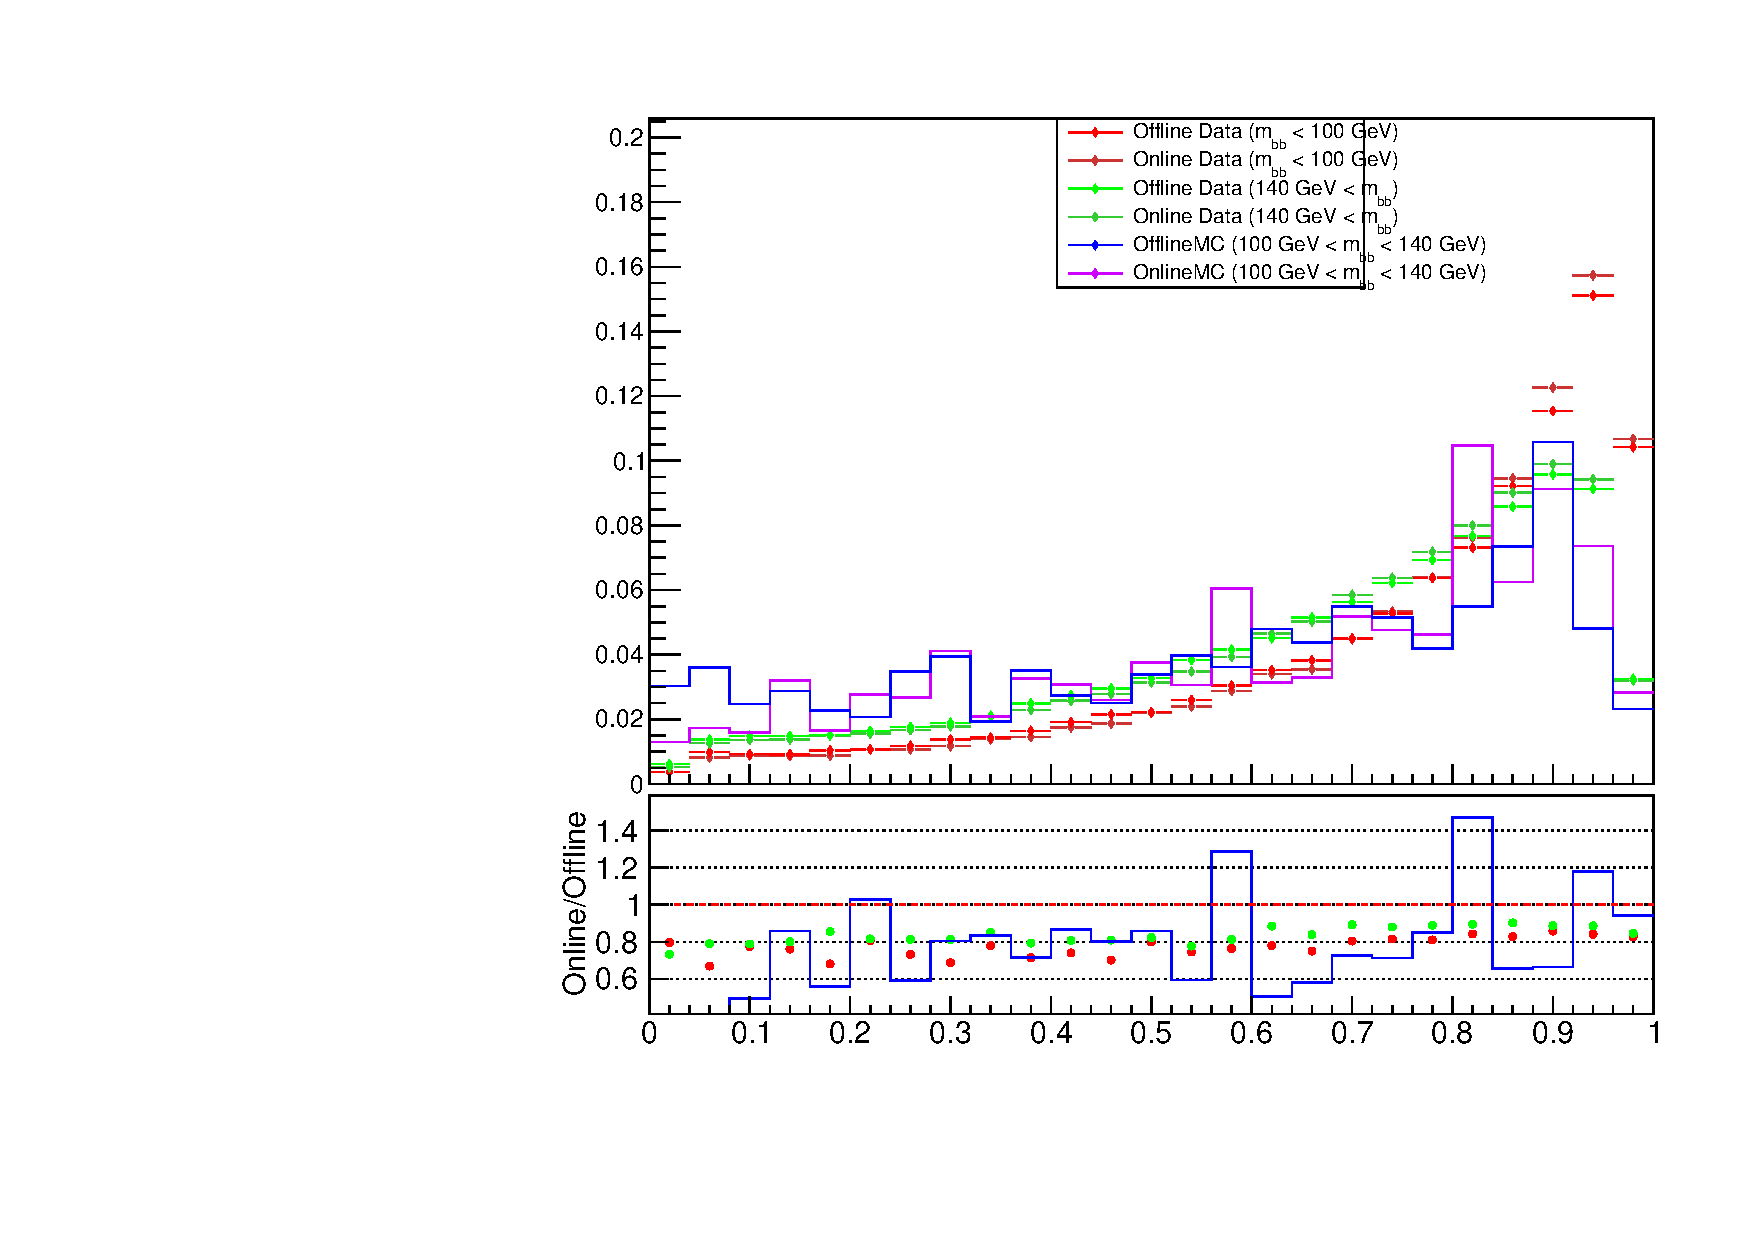
\includegraphics[width=1\linewidth]{ptbalance}
				\caption{}
				\label{fig:bdtptbalance}
			\end{minipage}
		\end{figure}


\section{Mbb Distribution}

		\begin{figure}[h]
			\centering
			\begin{minipage}[h]{0.45\linewidth}
				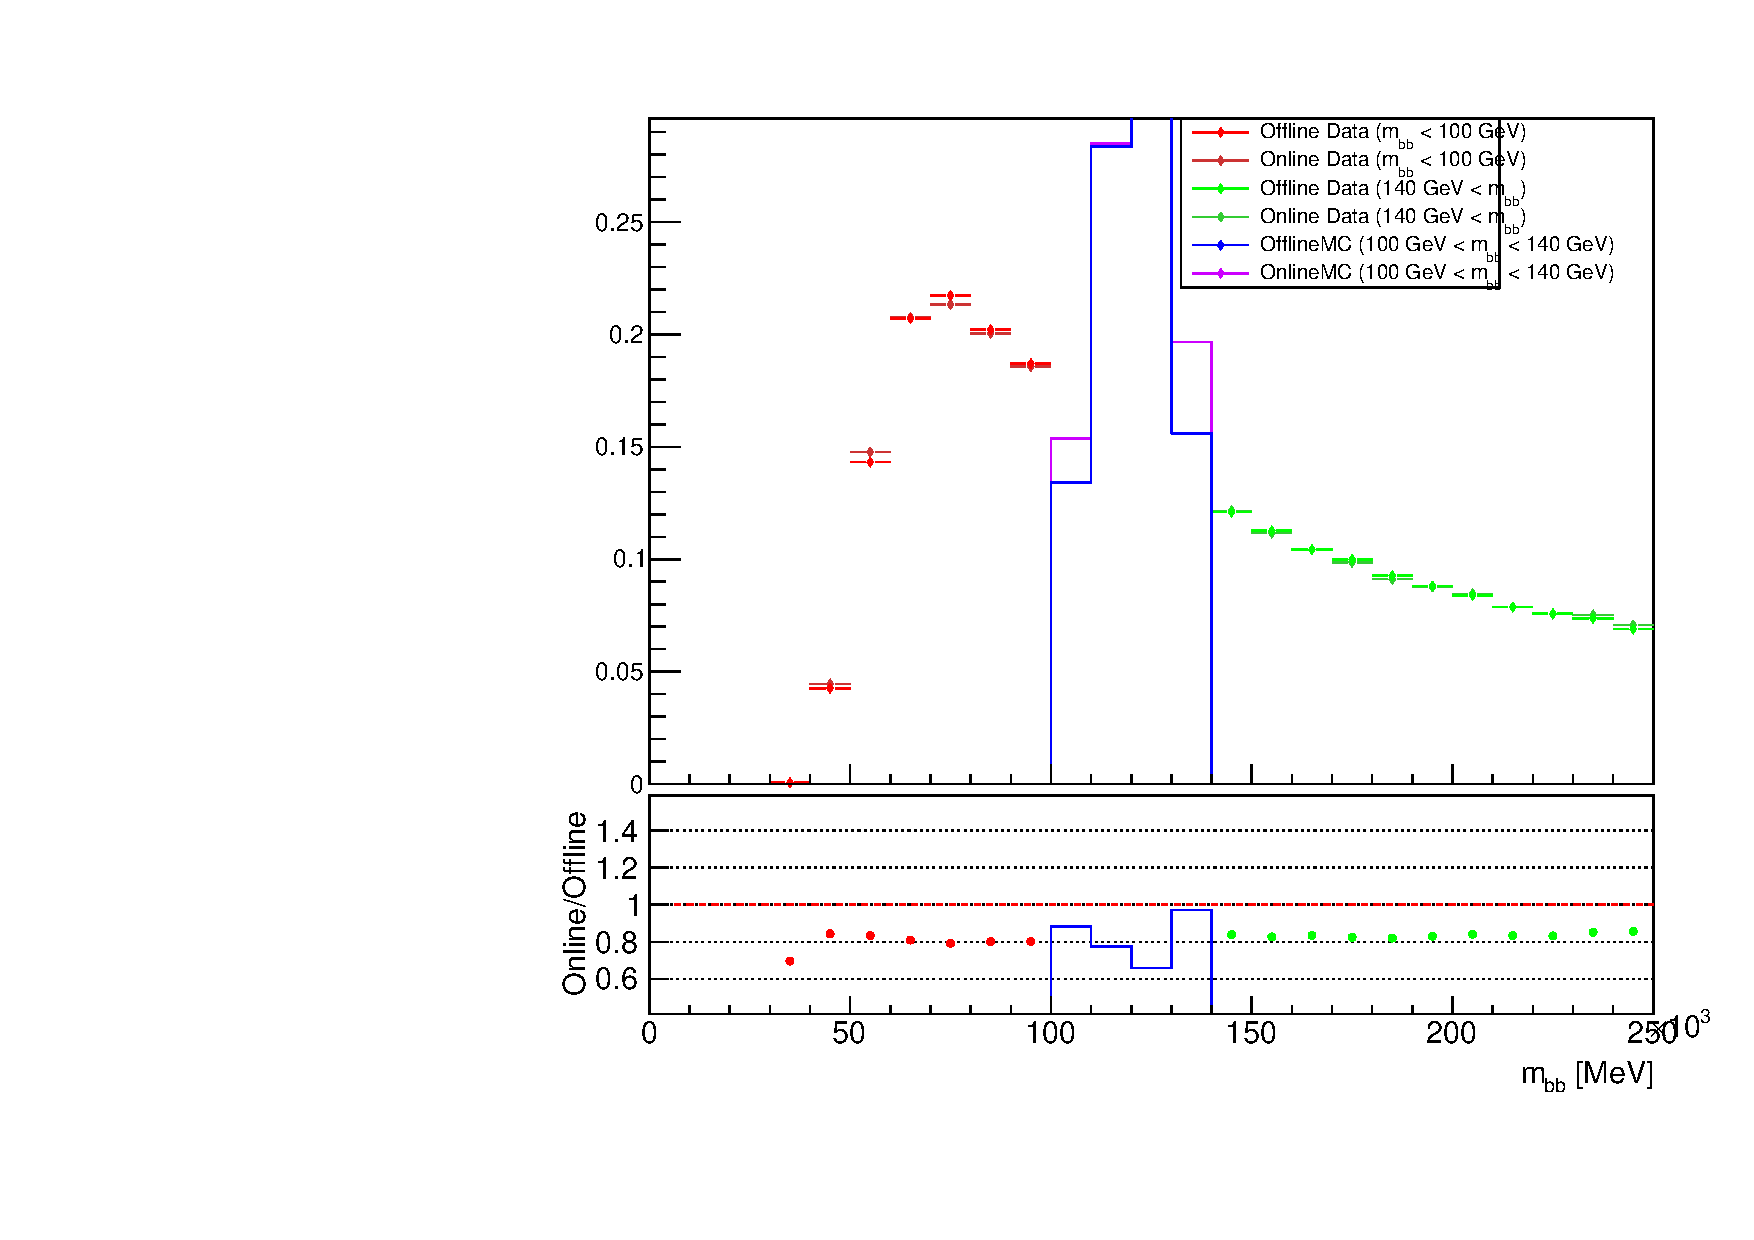
\includegraphics[width=1\linewidth]{mbb}
				\caption{}
				\label{fig:bdtmbb}
			\end{minipage}
			\quad
			\begin{minipage}[h]{0.45\linewidth}
				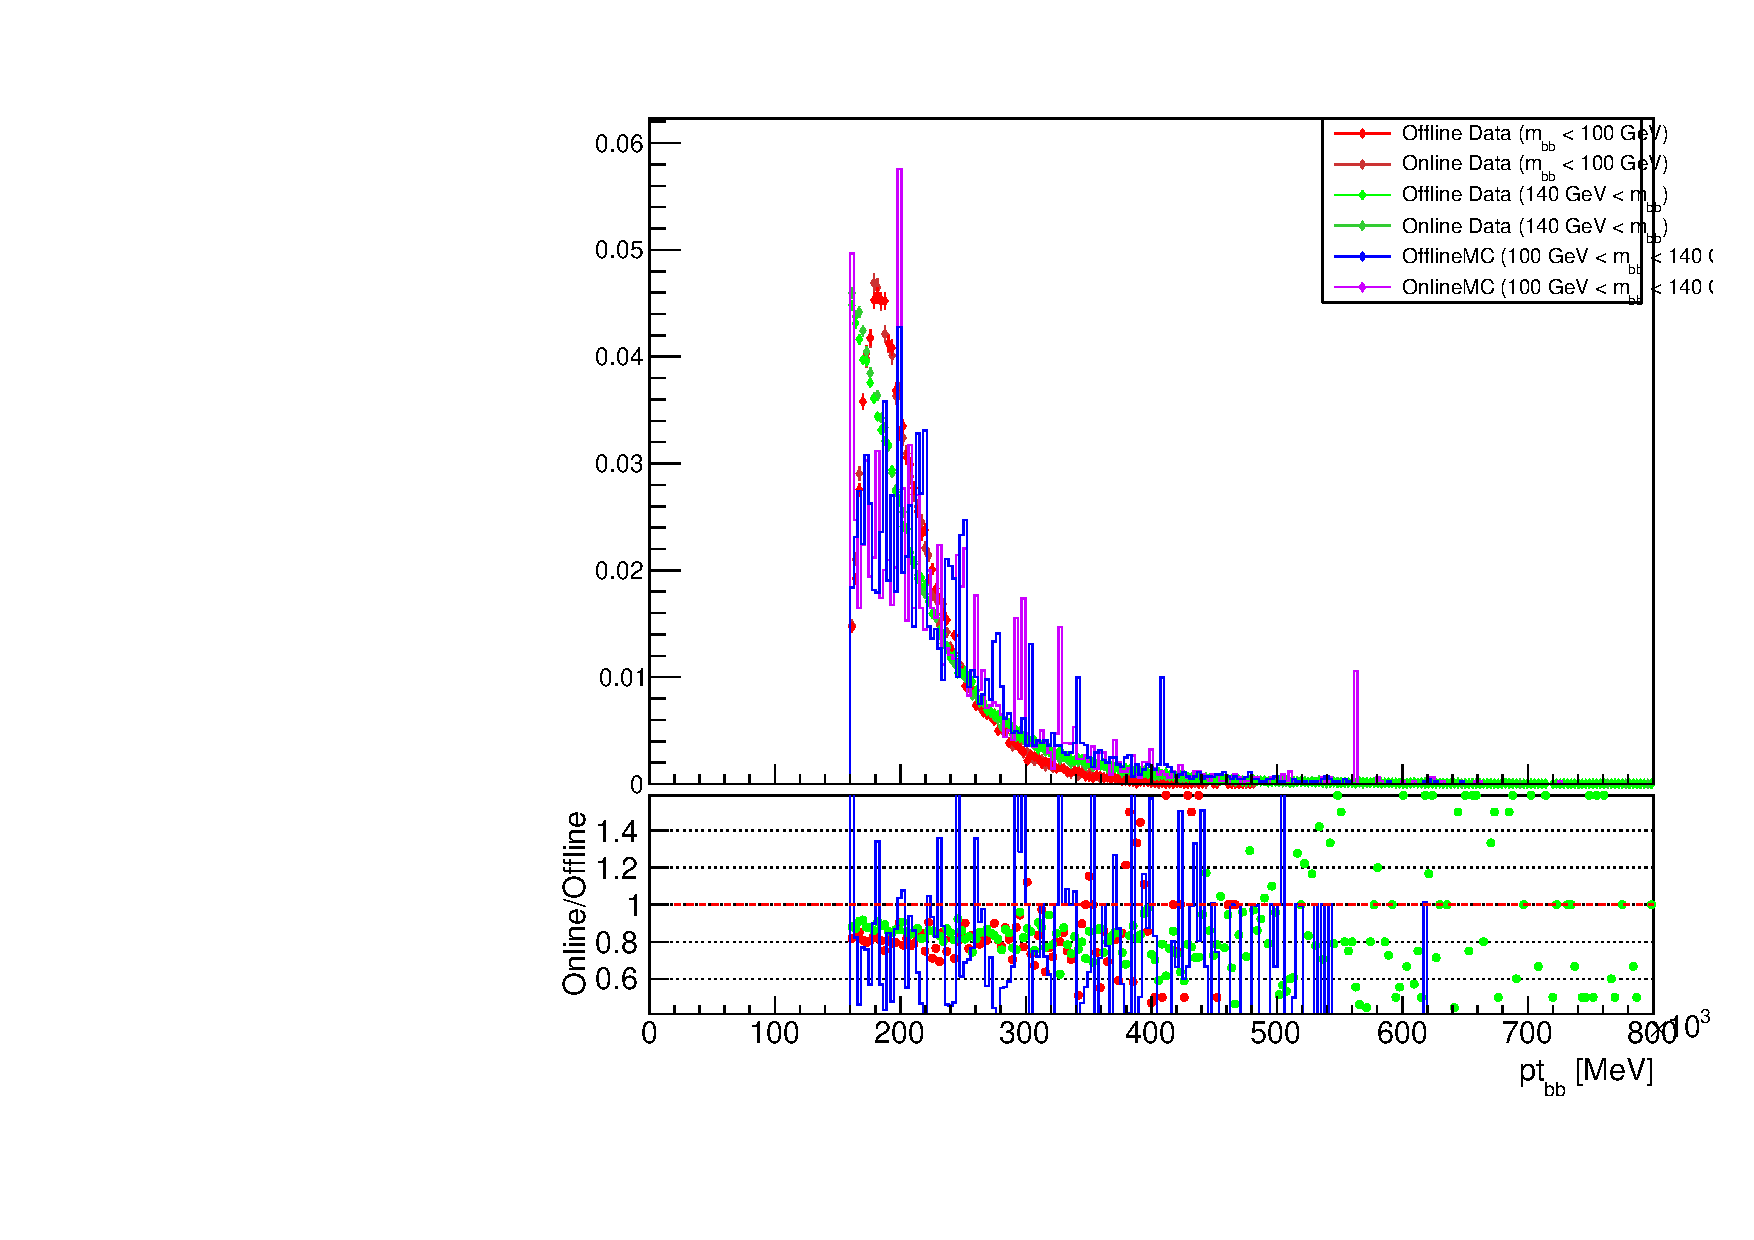
\includegraphics[width=1\linewidth]{ptbb}
				\caption{}
				\label{fig:bdtptbb}
			\end{minipage}
		\end{figure}

	Prior paper suggests this is the 'final' plot, a shape comparison between BDT influenced control and signal regions of the Mbb distribution. A little confused as to exactly what we need here.

\endinput
